% Created 2016-06-29 Wed 20:00
\documentclass[11pt]{amsart}
\usepackage[all]{pabmacros}
\usepackage[utf8]{inputenc}
\usepackage[T1]{fontenc}
\usepackage{fixltx2e}
\usepackage{graphicx}
\usepackage{longtable}
\usepackage{float}
\usepackage{wrapfig}
\usepackage[normalem]{ulem}
\usepackage{textcomp}
\usepackage{marvosym}
\usepackage[nointegrals]{wasysym}
\usepackage{latexsym}
\usepackage{amssymb}
\usepackage{amstext}
\usepackage{hyperref}
\tolerance=1000
\usepackage{amsmath}

\usepackage[bibstyle=alphabetic,citestyle=alphabetic,backend=bibtex]{biblatex}
\bibliography{refs}
\AtEveryBibitem{\clearfield{doi}}
\AtEveryBibitem{\clearfield{url}}
\AtEveryBibitem{\clearfield{issn}}
\renewcommand*{\bibfont}{\footnotesize}

\newcommand{\skel}[1]{\ensuremath{\operatorname{skel}({#1})}}

\DeclareMathOperator{\tangspeed}{v}
\DeclareMathOperator{\norfactor}{\lambda}
\DeclareMathOperator{\ineq_rel}{\simeq}
\DeclareMathOperator{\chordarcprofile}{\mathcal{Z}}
%\newcommand\holder{H\"older}
\DeclareMathOperator{\network}{\mathcal{N}}
\DeclareMathOperator{\corneranglespeed}{{\Delta v}}
\DeclareMathOperator{\tangindicator}{\iota}
\DeclareMathOperator{\norindicator}{\tau}


\usepackage{snapshot}

\author{Paul Bryan}
\address{Department of Mathematics, University of Queensland}
\email{pabryan@gmail.com}

\author{Mariel S\'aez}
\address{Facultad de Matematicas, Pontificia Universidad Cat\'olica de Chile, Avenida Vicu\'na Mackenna 4860, Macul, 6904441 Santiago, Chile}
\email{mariel@mat.puc.cl}

\keywords{Curvature flows, Distance comparison, Networks, curves}
\subjclass[2010]{53C44, 35K55, 58J35}
\date{}

\title[Dist. comp. for CSF networks]{A Distance Comparison Theorem For Curve Shortening Of Planar Networks} 
\hypersetup{
 pdfauthor={Paul Bryan},
 pdftitle={A distance comparison theorem for curve shortening of planar networks},
 pdfkeywords={},
 pdfsubject={},
 pdfcreator={Emacs 24.5.1 (Org mode 8.3.4)}, 
 pdflang={English}}

\begin{document}

\maketitle

\section{Introduction}
\label{sec:orgheadline1}
\section{Curve Shortening of Networks}
\label{sec:orgheadline5}

\subsection{Networks}
\label{sec:orgheadline2}

We consider networks with a single loop, \(\network = (\gamma, L)\) with \(L = \{L_i\}_{i=0}^{k-1}\). For us this means we have a piecewise smooth embedding for the loop:
\[
\gamma : \sphere^1 \to \RR^2.
\]
Let \(\{a_i\}_{i=0}^{k-1} \subset \sphere^{1}\) be such that \(\gamma\) is smooth on \(\sphere^1 \setdiff \{a_i\}\). We call \(\{a_i\}\) the nodes. We also have free ends \(L_i : [0, 1) \to \RR^2\) which are pairwise disjoint, smooth embeddings satisfying \(L_i(0) = \gamma(a_i)\), each curve \(L_i(0, 1)\) is disjoint from \(\gamma(\sphere^1)\), and either,
\begin{enumerate}
\item \(\lim_{x\to 1} |L_i(x)| = \infty\), or
\item \(\lim_{x\to 1} L_i(x) \in \bdry{\Omega}\) where \(\Omega \subset \RR^2\) is a compact, convex set with non-empty interior properly containing the loop, \(\gamma(\sphere^1) \subset \interior{\Omega}\).
\end{enumerate}
In either case, \(L_i(0,1)\) is contained in the region exterior to \(\gamma(\sphere^1)\).

Fixing an orientation on \(\sphere^1\) and parametrising the loop \(\gamma\) over \([0, 2\pi]\) we assume that,
\[
0 = a_0 < a_1 < \cdots < a_{k-1} < a_k = 2\pi
\]
and we always consider \(i\) modulo \(k\). Let us also write \(I_i = [a_{i-1}, a_i]\) and \(\gamma_i = \gamma|_{I_i}\) for the smooth connected arcs, which by assumption are smooth up to the boundary and satisfy \(\gamma_i(a_i) = \gamma_{i+1}(a_i)\) (\(i\) modulo \(k\)).

We also impose the \emph{triple condition} at the nodes: let
\[
\tang^{\pm} (a_i) = \lim_{x\to a_i^{\pm}} \frac{\gamma'(x)}{\|\gamma'(x)\|}, \quad \tang_{L_i}(0) = \frac{L_i'(0)}{\|L_i'(0)\|}
\]
denote respectively the tangents to the loop on either side of the node \(a_i\) and the tangent to the free curve \(L_i\) at \(a_i\). Then
\begin{equation}
\label{eq:triplecondition}
\ip{\tang^+(a_i)}{-\tang^-(a_i)} = \ip{\tang^{\pm}(a_i)}{\tang_{L_i}(0)} = - \frac{1}{2}.
\end{equation}
In other words, the tangents make equal angles \(2\pi/3\) at the nodes. See figure \ref{fg:network}.

\begin{figure}[htb]
\centering
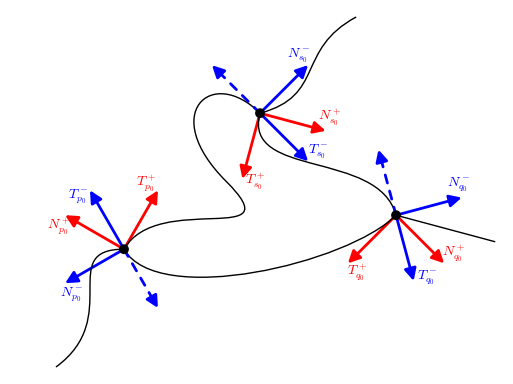
\includegraphics[width=.9\linewidth]{network}
\caption{A network with three nodes, $p_0, s_0, q_0$ satisfying the triple condition.}
\label{fg:network}
\end{figure}

Let us write \(\tang\) for the oriented, unit tangent and \(\nor\) for the unit, outer normal to \(\gamma\) on the smooth part \(\gamma^{\ast} = \gamma(\sphere^1\setdiff\{a_i\})\). Let us also write \(\tang_i\), \(\nor_i\) for the oriented unit, tangent and outer normal respectively to the connected smooth arcs \(\gamma_i\). At a node, write
\[
\nor_i^{\pm}(a_i) = \lim_{x\to a_i^{\pm}} \nor
\]
for the normals either side of the node \(a_i\). From the triple condition \eqref{eq:triplecondition} and the fact that each \(L_i\) is outward pointing, we have the relations
\begin{equation}
\label{eq:triplerelations}
\ip{-\tang^+}{\nor^-} = \ip{\tang^-}{\nor^+} = \ip{\nor_i^{\pm}}{\tang_i} = \frac{\sqrt{3}}{2}.
\end{equation}
See figure \ref{fg:node}.
\begin{figure}[htb]
\centering
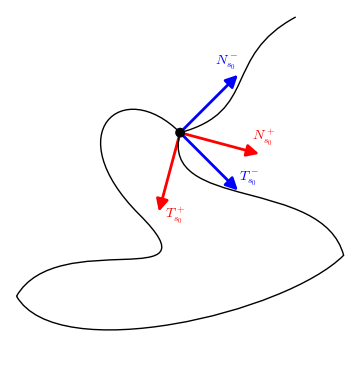
\includegraphics[width=.9\linewidth]{node}
\caption{A node with tangents and normals to the loop depicted.}
\label{fg:node}
\end{figure}

Analogously we also write \(\curvecurv\) for the curvature of \(\gamma^{\ast}\), \(\curvecurv_i\) for the curvature of the connected arcs \(\gamma_i\) and \(\curvecurv^{\pm}_i\) for the curvature of the loop on either side of the node \(a_i\). If needed, we will write \(\curvecurv_{L_i}\) for the curvature of the free curves \(L_i\). Our convention for the Frenet-Serret equations is that the curvature vector of a convex curve is inward pointing so that,
\begin{equation}
\label{eq:frenetserret}
\partial_s \tang = -\curvecurv \nor, \quad \partial_s \nor = \curvecurv \tang
\end{equation}
with \(s\) denoting the arc-length parameter.

\subsection{Curve Shortening Of Networks}
\label{sec:orgheadline3}

\begin{defn}
A smooth, one-parameter family \(\network_t = (\gamma_t, L_t)\), \(\gamma_t = (\gamma_i)_t\), \(L_t = (L_i)_t\), \(i=1,\cdots,k\) of embedded networks with one loop satisfying the triple condition \eqref{eq:triplecondition} evolves by \emph{curve shortening} if for each \(i\),
\begin{equation}
\label{eq:csf}
\left(\pd[\gamma_i]{t}\right)^{\perp} = -\curvecurv, \quad \text{and} \quad \left(\pd[L_i]{t}\right)^{\perp} = -\curvecurv.
\end{equation}
Here, for a vector field \(X\) along a curve, \(X^{\perp} = \ip{X}{\nor}\) denotes the outer normal component of \(X\) on the smooth part \(\network^{\ast} = (\gamma^{\ast}, L)\).
\end{defn}

In general, in order that for each \(t\), \(\network_t\) is an embedded network with one loop satisfying the triple condition \eqref{eq:triplecondition}, and evolving by the curve shortening flow \eqref{eq:csf}, there must be a non-zero tangential component of the speed. In other words,
\begin{equation}
\label{eq:csf_with_tang}
\pd[\gamma_i]{t} = -\curvecurv_i \nor_i + \tangspeed_i \tang_i, \quad \pd[L_i]{t} = -\curvecurv_{L_i} \nor_{L_i} + \tangspeed_{L_i} \tang_{L_i}
\end{equation}
where \(\tangspeed_i, \tangspeed_{L_i}\) are any smooth functions satisfying
\begin{equation}
\label{eq:speedcompatability}
-\curvecurv_i^+ \nor_i^+ + \tangspeed_i^+ \tang_i^+ = -\curvecurv_i^- \nor_i^- + \tangspeed_i^- \tang_i^- = -\curvecurv_{L_i} \nor_{L_i} + \tangspeed_{L_i} \tang_{L_i}
\end{equation}
at each node \(a_i\). Note that we are free to choose any smooth, \(\tangspeed_i, \tangspeed_{L_i}\) functions satisfying \eqref{eq:speedcompatability} without affecting the image of the evolving network in the plane.

Using the triple conditions \eqref{eq:triplecondition} \eqref{eq:triplerelations}, the first equality allows us to write \(v_i^{\pm}\) in terms of the curvatures \(\curvecurv_i^{\pm}\) and vice-versa:
\begin{align*}
\tangspeed_i^+ &= \ip{-\curvecurv_i^- \nor_i^- + \tangspeed_i^- \tang_i^-}{\tang_i^+} = \frac{\sqrt{3}}{2} \curvecurv_i^- + \frac{1}{2} \tangspeed_i^- \\
\tangspeed_i^- &= \ip{-\curvecurv_i^+ \nor_i^+ + \tangspeed_i^+ \tang_i^+}{\tang_i^-} = - \frac{\sqrt{3}}{2} \curvecurv_i^+ + \frac{1}{2} \tangspeed_i^+.
\end{align*}
Thus we have
\begin{equation}
\label{eq:tangspeedcurvture}
\tangspeed_i^+ = \frac{2}{\sqrt{3}} \curvecurv_i^- - \frac{1}{\sqrt{3}} \curvecurv_i^+, \quad \tangspeed_i^- = -\frac{2}{\sqrt{3}} \curvecurv_i^+ + \frac{1}{\sqrt{3}} \curvecurv_i^-
\end{equation}
and
\begin{equation}
\label{eq:curvturetangentialspeed}
\curvecurv_i^+ = -\frac{2}{\sqrt{3}} \tangspeed_i^- + \frac{1}{\sqrt{3}} \tangspeed_i^+, \quad \curvecurv_i^- = \frac{2}{\sqrt{3}} \tangspeed_i^+ - \frac{1}{\sqrt{3}} \tangspeed_i^-.
\end{equation}

Finally, let us define the corner tangential speed difference,
\begin{equation}
\label{eq:cornerspeed}
\corneranglespeed_i = \tangspeed_i^+ - \tangspeed_i^- = \frac{1}{\sqrt{3}} \left(\curvecurv_i^- + \curvecurv_i^+\right).
\end{equation}

\subsection{Basic Evolution Equations}
\label{sec:orgheadline4}

Let us assume that the loop \(\gamma_t\) is parametrised by \((u, t) \in [0, 2\pi] \times [0, T)\). Throughout we denote by \(s\) the arc length parameter so that
\[
\partial_s = \frac{1}{\abs{\gamma_t'}} \partial_u, \quad ds = \abs{\gamma_t'} du
\]
where primes denote differentiation with respect to \(u\).

The evolution of geometric quantities under the Curve Shortening Flow is the same for networks as in the smooth case. This is immediate for any pointwise quantities, and we record the required equations in a lemma for later convenience.

\begin{lemma}
\label{lem:basic_evolution}
The following evolution equations hold:
\begin{enumerate}
\item \(\pd[ds]{t} = (\partial_s \tangspeed - \curvecurv^2) ds\)
\item \([\partial_t, \partial_s] = -(\partial_s \tangspeed - \curvecurv^2) \partial_s\)
\item \(\pd[\tang]{t} = -(\partial_s \curvecurv + \tangspeed\curvecurv) \nor\)
\item \(\pd[\nor]{t} = (\partial_s \curvecurv + \tangspeed\curvecurv) \tang\)
\item \(\pd[\curvecurv]{t} = \partial_s^2 \curvecurv + \curvecurv^3 + \tangspeed \partial_s \curvecurv\).
\end{enumerate}
\end{lemma}

Let us now state the definitions we use for intrinsic and extrinsic distances. Note in particular, the intrinsic distance we use is oriented which is for convenience and makes for slightly cleaner exposition later.

\begin{defn}
\label{defn:dist}
Let \((p,q) \in \gamma \times \gamma\). The \emph{extrinsic distance} is defined to be,
\[
d_t(p, q) = \|\gamma_t(q) - \gamma_t(p)\|.
\]
The \emph{oriented intrinsic distance} or \emph{oriented arc length} is defined to be,
\[
\ell_t(p, q) = \int_{\gamma_t} ds_t = \int_p^{a_i} ds_t + \sum_{m=i+1}^{j-1} \int_{a_{m-1}}^{a_m} ds_t + \int_{a_{j-1}}^q ds_t
\]
where \(p \in I_i = [a_{i-1}, a_i]\), \(q \in I_j = [a_{j-1}, a_j]\) and \(i,j\) are taken modulo \(k\).
\end{defn}

Note that by oriented, we mean the length along \(\gamma\) from \(p\) to \(q\) in the chosen orientation of \(\gamma\). For \(p > q\), (for the moment not taking \(i,j\) modulo \(k\)),
\[
\ell(p, q) = \int_p^{a_i} ds_t + \sum_{m=i+1}^{k} \int_{a_{m-1}}^{a_m} ds_t + \sum_{m=1}^{j-1} \int_{a_{m-1}}^{a_m} ds_t + \int_{a_{j-1}}^q ds_t
\]
and \(\ell(p, q)\) is always non-negative. Note also that with our definition \(\ell\) is not symmetric but satisfies,
\begin{equation}
\label{eq:ell_symmetry}
\ell(q, p) = 2\pi L - \ell(p, q).
\end{equation}
The usual intrinsic distance between \(p\) and \(q\), denoted here by \(\tilde{\ell}(p, q)\), satisfies
\[
\tilde{\ell}(p, q) = \min\{\ell(p, q), \ell(q, p)\} = \min\{\ell(p, q), 2\pi L - \ell(p, q)\}.
\]

Let us also define
\begin{equation}
\label{eq:w}
w(p, q) = \frac{\gamma(q) - \gamma(p)}{d(p,q)},
\end{equation}
the unit vector pointing from \(p\) to \(q\).

Later we will only require the evolution of the extrinsic and intrinsic distances at smooth points.

\begin{lemma}
\label{lem:distance_evolution}

Let \((p,q) \in \gamma_t^{\ast}\) be smooth points. Then,
\begin{align*}
\partial_t d_t(p, q) &= -\curvecurv_q \ip{\nor_q}{w} + \curvecurv_p \ip{\nor_p}{w} + \tangspeed_q \ip{\tang_q}{w} - \tangspeed_p \ip{\tang_p}{w}, \\
\partial_t \ell_t(p, q) &= - \int_p^q \curvecurv^2 ds + \tangspeed(q) - \tangspeed(p) - \sum_{m=i}^{j-1} \corneranglespeed_m \\
\intertext{and}
\partial_t L &= - \int_{\gamma} \curvecurv^2 ds - \sum_{m=i}^{k} \corneranglespeed_m.
\end{align*}
\end{lemma}

\begin{proof}
From the evolution equation \eqref{eq:csf_with_tang} we obtain,
\[
\begin{split}
\partial_t \ip{\gamma(q) - \gamma(p)}{\gamma(q) - \gamma(p)} &= 2 \ip{-\curvecurv(q) \nor(q) + \tangspeed(q) \tang(q)}{\gamma(q) - \gamma(p)} \\
&\quad  - 2 \ip{-\curvecurv(p) \nor(p) + \tangspeed(p) \tang(p)}{\gamma(q) - \gamma(p)}.
\end{split}
\]
The evolution of \(d = \left(\ip{\gamma(q) - \gamma(p)}{\gamma(q) - \gamma(p)}\right)^{1/2}\) follows by the chain rule and the definition of \(w\).

Using the evolution of \(ds\) from Lemma \ref{lem:basic_evolution},
\begin{align*}
\partial_t \ell(p,q) &= \partial_t \int_p^{a_i} ds_t + \sum_{m=i+1}^{j-1} \partial_t \int_{a_{m-1}}^{a_m} ds_t + \partial_t  \int_{a_{j-1}}^q ds_t \\
&= \int_p^{a_i} (\partial_s \tangspeed - \curvecurv^2 )ds_t + \sum_{m=i+1}^{j-1} \int_{a_{m-1}}^{a_m} (\partial_s \tangspeed - \curvecurv^2 )ds_t + \int_{a_{j-1}}^q (\partial_s \tangspeed - \curvecurv^2) ds_t \\
&= -\int_p^q \curvecurv^2 ds + \tangspeed_i^- - \tangspeed(p) + \sum_{m=i+1}^{j-1} \tangspeed_m^- - \tangspeed_{m-1}^+ + \tangspeed(q) - \tangspeed_{j-1}^+ \\
&= -\int_p^q \curvecurv^2 ds + \tangspeed(q) - \tangspeed(p) + \sum_{m=i}^{j-1} \tangspeed_m^- - \tangspeed_m^+.
\end{align*}
The evolution of \(\ell\) follows immediately from the definition of \(\corneranglespeed\), while the evolution of \(L\) follows by taking \(p=a_0=a_k=q\).
\end{proof}

\begin{remark}
Unlike the smooth case, it is a-priori possible that length actually increases under the network flow. See also the remark below following Lemma \ref{lem:dtA}.
\end{remark}

It's also worth remarking that the evolution of the extrinsic distance does not feel the presence of the nodes, while the intrinsic length, being forced to traverse the nodes does. Next we compute the evolution of enclosed area, which by Stokes' theorem may be computed as an integral along \(\gamma\) and hence also feels the presence of the nodes.

\begin{lemma}
\label{lem:dtA}
The enclosed area evolves by,
\[
\partial_t \area = - \left(2 - \tfrac{k}{3}\right)\pi.
\]
\end{lemma}

\begin{proof}
We use the formula,
\[
\area = \frac{1}{2} \sum_{i=1}^k \int_{a_{i-1}}^{a_i} \ip{\gamma}{\nor} ds
\]
to compute,
\[
\begin{split}
\partial_t \area &= \frac{1}{2} \sum_{i=1}^k \int_{a_{i-1}}^{a_i} \ip{\partial_t \gamma}{\nor} ds \\
&\quad + \frac{1}{2} \sum_{i=1}^k \int_{a_{i-1}}^{a_i} \ip{\gamma}{\partial_t \nor} ds + \ip{\gamma}{\nor} \partial_t ds
\end{split}
\]

The first term is,
\[
\frac{1}{2} \sum_{i=1}^k \int_{a_{i-1}}^{a_i} \ip{\partial_t \gamma}{\nor} ds = \frac{1}{2} \sum_{i=1}^k \int_{a_{i-1}}^{a_i} \ip{-\curvecurv \nor + \tangspeed \tang}{\nor} ds = -\frac{1}{2} \int_{\gamma} \curvecurv.
\]

Using the evolution equations in Lemma \ref{lem:basic_evolution} and the Frenet-Serret equations \eqref{eq:frenetserret}, the integrand in the second term is,
\[
\begin{split}
\ip{\gamma}{\partial_t \nor} ds + \ip{\gamma}{\nor} \partial_t ds &= \ip{\gamma}{(\partial_s \curvecurv + \tangspeed \curvecurv)\tang} ds + \ip{\gamma}{\nor} (\partial_s \tangspeed - \curvecurv^2) ds \\
&= \ip{\gamma}{\partial_s(\curvecurv\tang) + \curvecurv^2 \nor} ds + \tangspeed\curvecurv \ip{\gamma}{\tang} ds \\
&\quad + \ip{\gamma}{\partial_s (\tangspeed \nor) - \tangspeed \curvecurv \tang} ds - \curvecurv^2 \ip{\gamma}{\nor} ds \\
&= \partial_s \ip{\gamma}{\curvecurv\tang + \tangspeed \nor} ds - \ip{\tang}{\curvecurv \tang + \tangspeed \nor} ds \\
&= \partial_s \ip{\gamma}{\curvecurv\tang + \tangspeed \nor} ds - \curvecurv ds.
\end{split}
\]
Integrating we obtain,
\begin{equation}
\label{eq:dtA_prelim}
\begin{split}
\partial_t \area &= -\int_{\gamma} \curvecurv ds + \frac{1}{2} \sum_{i=1}^k \ip{\gamma(a_i)}{\curvecurv_i^- \tang_i^- + \tangspeed_i^- \nor_i^-} - \ip{\gamma(a_{i-1})}{\curvecurv_{i-1}^+ \tang_{i-1}^+ + \tangspeed_{i-1}^+ \nor_{i-1}^+} \\
&= - \left(2 - \tfrac{k}{3}\right)\pi - \frac{1}{2} \sum_{i=1}^k \ip{\gamma(a_i)}{\curvecurv_i^+ \tang_i^+ + \tangspeed_i^+ \nor_i^+ - \curvecurv_i^- \tang_i^- - \tangspeed_i^- \nor_i^-},
\end{split}
\end{equation}
since the turning angle at each node is \(\theta_i = \arccos \ip{\tang^+}{\tang^-} = \tfrac{\pi}{3}\) and since the sum is taken modulo \(k\).

As to the sum, recall the compatibility conditions
\[
\ip{\tang^+_i}{\tang^-_i} = \ip{\nor^+_i}{\nor^-_i} = \frac{1}{2} \tag{\ref{eq:triplecondition} revisited}
\]
gave rise to
\[
\ip{-\tang^+_i}{\nor^-_i} = \ip{\tang^-_i}{\nor^+_i} = \frac{\sqrt{3}}{2} \tag{\ref{eq:triplerelations} revisited}.
\]
Then we have
\[
\tang^-_i = \frac{1}{2} \tang^+_i + \frac{\sqrt{3}}{2} \nor^+_i, \quad \nor^-_i = -\frac{\sqrt{3}}{2} \tang^+_i + \frac{1}{2} \nor^+_i
\]
and
\[
\tangspeed_i^+ = \frac{2}{\sqrt{3}} \curvecurv_i^- - \frac{1}{\sqrt{3}} \curvecurv_i^+, \quad \tangspeed_i^- = -\frac{2}{\sqrt{3}} \curvecurv_i^+ + \frac{1}{\sqrt{3}} \curvecurv_i^- \tag{\ref{eq:tangspeedcurvture} revisited}.
\]

Therefore
\[
\begin{split}
& \curvecurv_i^+ \tang_i^+ + \tangspeed_i^+ \nor_i^+ - \curvecurv_i^- \tang_i^- - \tangspeed_i^- \nor_i^- \\
&\quad = \curvecurv_i^+ \tang_i^+ + \left(\frac{2}{\sqrt{3}} \curvecurv_i^- - \frac{1}{\sqrt{3}} \curvecurv_i^+\right) \nor_i^+ \\
&\quad\quad - \curvecurv_i^- \left(\frac{1}{2} \tang^+_i + \frac{\sqrt{3}}{2} \nor^+_i\right) - \left(-\frac{2}{\sqrt{3}} \curvecurv_i^+ + \frac{1}{\sqrt{3}} \curvecurv_i^-\right)\left(-\frac{\sqrt{3}}{2} \tang^+_i + \frac{1}{2} \nor^+_i\right) \\
&\quad = \left(\curvecurv_i^+ - \frac{1}{2} \curvecurv_i^- - \curvecurv_i^+ + \frac{1}{2}\curvecurv_i^-\right) \tang^+_i + \left(\frac{2}{\sqrt{3}} \curvecurv_i^- - \frac{1}{\sqrt{3}} \curvecurv_i^+ - \frac{\sqrt{3}}{2} \curvecurv_i^- + \frac{1}{\sqrt{3}} \curvecurv_i^+ - \frac{1}{2\sqrt{3}} \curvecurv_i^-\right) \nor^+_i \\
&\quad = 0.
\end{split}
\]
Thus the sum in equation \eqref{eq:dtA_prelim} vanishes giving the result.
\end{proof}

\begin{remark}
\begin{enumerate}
\item The sum on the right hand side of the evolution of \(\area\) will generally not vanish. In certain symmetric cases, such as the convex, symmetric, lens shaped networks studied in \cite{MR2763716}, the symmetry does in fact cause the terms to cancel. In that situation, there are two nodes \(a_1, a_2\) and the curvatures \(\curvecurv^{\pm}_1 = \curvecurv^{\pm}_2 = \kappa\) are all equal. Such symmetries, being invariance under ambient isometry, are of course preserved along the flow. The presence of the nodes is still felt in these cases through \(\partial_t \area = -(2- \tfrac{k}{3})\pi\) (as opposed to \(\partial_t \area = - 2\pi\) in the smooth case) but only the number of nodes \(k\), is relevant.

\item From the term, \(-(2- \tfrac{k}{3})\pi\) in \(\partial_t \area\), we see that increasing the number of nodes tends to slow the contraction. In fact, it is quite possible (especially for \(k > 6\)) that \(\partial_t \area > 0\), whence \(\gamma\) expands. Compare with the smooth curve shortening flow where \(\partial_t \area = - 2\pi < 0\).

\item In the particular case \(k = 6\), there exist static solutions enclosing area \(A\) for every \(A > 0\). These are obtained by letting \(\gamma\) be any equi-angular hexagon, and the \(L_i\) straight lines. On the other hand, by Gauss-Bonnet, and the triple condition we have \(\int_{\gamma} \curvecurv = (2 - \tfrac{k}{3}) \pi\), so that \(\gamma\) is polygonal if and only if \(\curvecurv \equiv 0\), if and only if \(k = 6\) and \(\gamma\) is an equi-angular hexagon. Given such an initial, equi-angular hexagon \(\gamma\), if the \(L_i\) are not straight lines, then the curvature at the node will drive \(\gamma\) away from a hexagon. Even if the curvature of the \(L_i\) vanishes in a neighbourhood of node, but is not identically zero, we expect infinite propagation speed to force the curvature at the node away from zero and again disturb the hexagon. Thus the static solutions are unstable under small perturbations.

\end{enumerate}
\end{remark}

\textcolor{red}{HERE ARE THE EXTRA COMPUTATIONS}
\begin{lemma}
Assume that the arcs $L_i$ have bounded length and let
$L_T$ be the
total length of the network $N_t$ (i.e.
 the length of the loop plus the length of $L_i$). Then 
  $$\partial_t L_T=-\int_{N_t}k^2 ds.$$


\begin{proof}
As before we have that
$$\partial_t L_T=-\int_{N_t}k^2 ds+\sum_i \Delta v_i + v_{L_i}(1)-v_{L_i}(0).$$

If the point at the boundary is fixed we have that $v_{L_i}(1)=0$. 
Then the claim follows from showing that 
$\Delta v_i-v_{L_i}(0)=0$.

From \eqref{eq:speedcompatability}
we have that
\begin{align*}
\tangspeed_i^+ &= \ip{-\curvecurv_i^- \nor_i^- + \tangspeed_i^- \tang_i^-}{\tang_i^+} = \frac{\sqrt{3}}{2} \curvecurv_i^- + \frac{1}{2} \tangspeed_i^- \\
\tangspeed_i^- &= \ip{-\curvecurv_i^+ \nor_i^+ + \tangspeed_i^+ \tang_i^+}{\tang_i^-} = - \frac{\sqrt{3}}{2} \curvecurv_i^+ + \frac{1}{2} \tangspeed_i^+
\\
\tangspeed_i^+ &= \ip{-\curvecurv_{L_i} \nor_{L_i} + \tangspeed_{L_i} \tang_{L_i}}{\tang_i^+} = \frac{\sqrt{3}}{2} \curvecurv_{L_i} - \frac{1}{2} \tangspeed_{L_i}\\
\tangspeed_i^- &= \ip{-\curvecurv_{L_i} \nor_{L_i} + \tangspeed_{L_i} \tang_{L_i}}{\tang_i^-} =  \frac{\sqrt{3}}{2} \curvecurv_{L_i} + \frac{1}{2} \tangspeed_{L_i}\\
\tangspeed_{L_i} &= \ip{-\curvecurv_i^- \nor_i^- + \tangspeed_i^- \tang_i^-}{\tang_{L_i}} = - \frac{\sqrt{3}}{2} \curvecurv_i^- + \frac{1}{2} \tangspeed_i^-\\
\tangspeed_{L_i} &= \ip{-\curvecurv_i^+ \nor_i^+ + \tangspeed_i^+ \tang_i^+}{\tang_{L_i}} = - \frac{\sqrt{3}}{2} \curvecurv_i^+ - \frac{1}{2} \tangspeed_i^+.
\end{align*}

Then taking $2(\tangspeed_i^--
\tangspeed_i^+-\tangspeed_{L_i})$
from the right hand side (and being careful with the signs of the other side) we get the desired result.

\end{proof}
\end{lemma}
\begin{remark}
If for $p=\gamma(x,t)$ and $q=\gamma(y,t)$ we define the function 
$$\tilde{\ell}=\ell(p,q)+\sum_{\{i:x\leq a_i <y\}}|L_i|,$$
and $\ell$ is the distance oriented in some direction, then
$$\partial_t\tilde{\ell}(p,q)=-\int_p^qk^2- \sum_{\{i:x\leq a_i <y\}}\int_{L_i} k^2$$


This function is not continuous in $p$ and $q$ as one of them approaches a node, but it can be made lower or upper semi-continuous and there is a theory of viscosity solutions for such class of functions. The function is not symmetric respect to the half of the total distance either.
\end{remark}
\section{Self Similar Solutions}
\label{sec:self_similar}

Our comparison functions are constructed from the profile of self-simlar solutions and we collect here the basic facts about such solutions.

\begin{defn}
\label{defn:self_simlar}
A solution, \(\sigma\) of the network curve shortening flow is self-similar if there exists a point \(x_0 \in \RR^2\) and a smooth function \(\lambda : [0, T) \to \RR_+\) such that
\[
\sigma_t = \lambda(t) (\sigma_0 - x_0).
\]
\end{defn}
Since the network curve shortening flow is invariant under ambient isometry, we can and will assume that \(x_0 = (0, 0)\) is the origin.

A rather useful notion we introduce here is that of the \emph{skeleton} of a network.

\begin{defn}
\label{defn:skeleton}
Let \(\gamma\) be the loop of network with one loop and nodes \(\{x_1, \cdots, x_k\}\). The \emph{skeleton} of \(\gamma\) is the network \(\skel{\gamma}\) with nodes \(\{x_1, \cdots, x_k\}\), a loop formed by the edges \(e_i = \overline{x_ix_{i+1}}\) and unbounded lines tangent to \(L_i\) the unbounded curve for \(\gamma\) at the node \(x_i\).
\end{defn}

\begin{remark}
The skeleton of \(\gamma\) will not in general satisfy the triple condition. Neither need it be embedded! Nevertheless, the skeleton of \(\gamma\) is always homotopic to \(\gamma\) where we insist that homotopies of networks map nodes homeomorphically to nodes with respect to the discrete topology on the nodes.
\end{remark}

We are particularly interested in those networks with skeleton a regular polygon.

\begin{defn}
A network with one loop is call \emph{regular polygonal} if it's skeleton is a regular polygon.
\end{defn}

The skeletons of various regular polygonal networks along with the triple condition highlighted are show in figure \ref{fg:regularpolygon}.

\begin{figure}[htb]
\centering
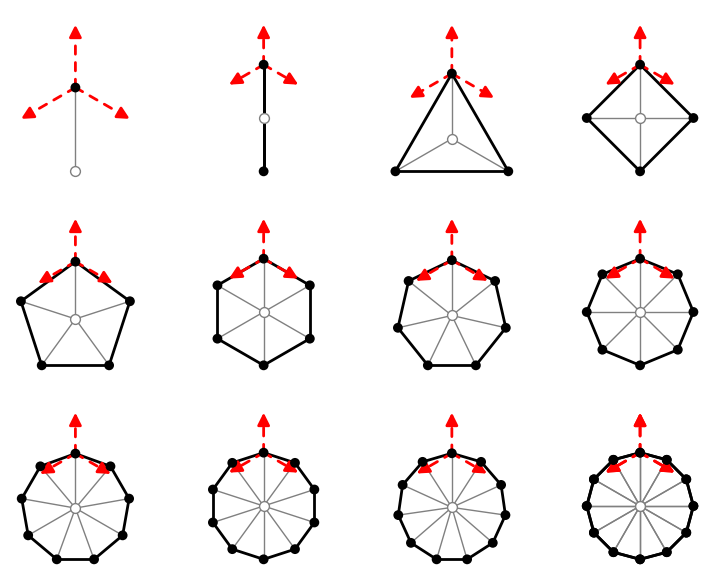
\includegraphics[width=.9\linewidth]{regularpolygon}
\caption{The skeleton of regular polygonal networks with triple condition highlighted.}
\label{fg:regularpolygon}
\end{figure}

Self-similar solutions with a single loop have been classified in \cite{MR2340176}. Including the smooth case as having \(k=0\) nodes and making use of the classification from \cite{MR845704} then the classification may be stated as follows:

\begin{theorem}[\cite{MR2340176,MR845704}]
For each \(k = 0, 1, 2, \cdots\) there exists a unique, regular polygonal, self-similar network \(\sigma_k\) with \(k\) nodes whose unbounded curves are straight lines. In both the cases \(k = 2,3\) there exists precisely one other self-similar solution known as the ``fish'' and the ``rocket'' for \(k = 2\) and \(k = 3\) respectively. For any other \(k\), there are no other self-similar solutions besides the regular polygonal self-similar network.
\end{theorem}

\begin{remark}
For \(k = 0\), there are no nodes, and the self-similar solution is the circle. For \(k = 1\), the skeleton is a single node with a half-line emanating from it. This self-similar solution is known is known as the ``Brakke Spoon''. For $k=2$, the skeleton is a line with two points on it. The self-similar solution is known as the ``Lens''.
\end{remark}

Some of the self similar regular polygonal networks are shown in \ref{fg:selfsimilarregularpolygon}.

\begin{figure}[htb]
\centering
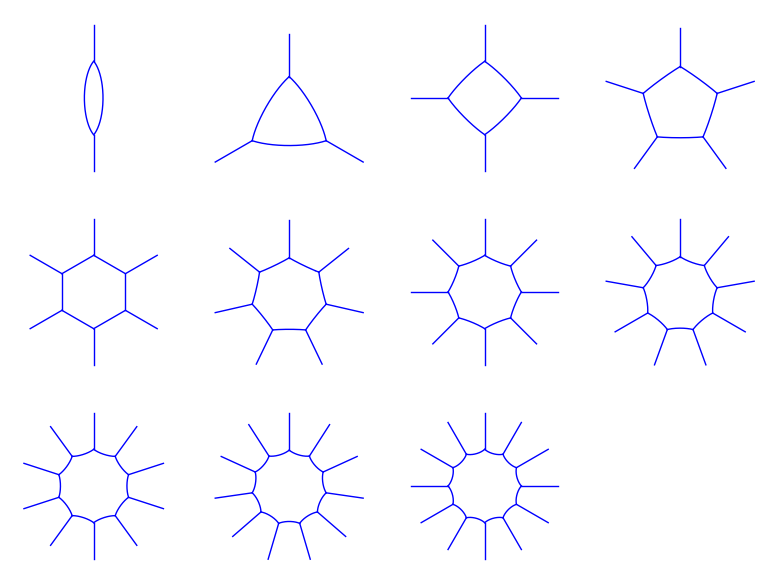
\includegraphics[width=.9\linewidth]{selfsimilarregularpolygon}
\caption{Self similar regular polygonal networks.}
\label{fg:selfsimilarregularpolygon}
\end{figure}

Let us now give a fairly explicit description of the the regular polygonal self-similar network, \(\sigma_k\). First, it is symmetric under the cyclic group \(C_k\) of rotations generated by the rotation of angle \(2\pi/k\) and symmetric under reflection across a line of symmetry bisecting an edge of the skeleton's regular polygon (and therefore all such lines of symmetry by the rotation invariance). That is, \(\sigma_k\) is invariant under the Dihedral group \(D_k\). Thus by the rotation invariance, each arc \(\gamma_i\) joining \(x_i\) to \(x_{i+1}\) is congruent to every other arc \(\gamma_j\) by a rotation of angle \(2\pi \ell/k\) where \(\ell = j - i\). Thus we may speak of \emph{the} arc of a regular polygonal self-similar network. This arc is an arc of an Abresch-Langer curve (see \cite{MR845704,MR2931330}). It may be written as a normal graph over the edge \(e_i\), symmetric about the mid-point of \(e_i\) by the reflection invariance.

For \(0 \leq k < 6\), the arc has strictly positive curvature with respect to the outer unit normal, for \(k = 6\) the arc \(e_i\) is equal to the edge \(e_i\), and for \(k > 6\) the arc \(\gamma_i\) has strictly negative curvature with respect to the outer unit normal.

We write the quantities from \eqref{eq:Q} and \eqref{eq:delQ} as
\begin{align*}
\bar{Q}_0 &= \int_{\gamma_0} \kappa^2 ds - \frac{1}{\sqrt{3}} \sum_{m=1}^{k} \kappa_i^+ + \kappa_i^-.\\
\Delta Q_0 (x) &= \int_{p_0}^{q_0} \kappa^2 ds - \frac{1}{\sqrt{3}} \sum_{m=i}^{j-1} \kappa_i^+ + \kappa_i^-.
\end{align*}
where $(p_0, q_0)$ are optimal points such that $\ell(p_0, q_0) = \frac{L}{2\pi} x$. Note that $\tfrac{L}{4\pi^2} \bar{Q}_0$ is a fixed, scale invariant number depending only on $\sigma$ and $\tfrac{L}{2\pi} \Delta Q_0(x)$ is a scale invariant function depending only on $\sigma$.

To be concrete, let us parametrise \(e_i = \overline{x_i x_{i+1}}\) over \([-1/2, 1/2]\) by
\[
x \in [-1/2, 1/2] \mapsto \left(\frac{1}{2} + x\right) x_i + \left(\frac{1}{2} - x\right) x_{i+1}.
\]
The unit normal to \(e_i\) is
\[
\nu_i = \frac{x_i + x_{i+1}}{\abs{x_i + x_{i+1}}}.
\]

Then \(\gamma_i\) is parametrised by
\[
x \in [-1/2, 1/2] \mapsto e_i(x) + u(x) \nu_i
\]
where \(u : [-1/2, 1/2]\) is the unique solution of the boundary value problem
\begin{equation}
\label{eq:self_similar_graph}
\begin{cases}
u'' &= \bar{Q}_0 (xu' - u)(1 + (u')^2) \\
u(-1/2) &= u(1/2) = 0 \\
u'(-1/2) &= -u'(1/2) = \pm \sqrt{\cos^{-2} \left(\frac{\pi}{k}(6 - k)\right) - 1}.
\end{cases}
\end{equation}
where we have \(+\) when \(k \leq 6\) and we have \(-\) for \(k \geq 6\). Note that \(u\) is necessarily symmetric about \(x = 0\): \(u(-x) = u(x)\).

Although the existence of regular polygonal self-similar networks is known, we give of a proof of existence here explicitly based on the graphs \(u\) solving \eqref{eq:self_similar_graph}. Note that for \(k = 0\), we obtain the circle as proven in \cite{MR845704}, for \(k = 1\) we obtain the Brakke spoon as obtained in \cite{}, for \(k = 2\), we obtain the Lens shaped network as obtained in \cite{MR2763716}. More generally, for all \(k > 0\), we obtain those solutions obtained \cite{MR2340176}.

\begin{lemma}
For each \(k = 0, 1, 2, \cdots\), there exists a homothetic solution of the network curve shortening flow with \(k\) nodes whose skeleton is the regular polygon of \(k\) nodes and that is symmetric under the Dihedral group, $D_k$ of symmetries of it's regular polygon skeleton. For \(0 \leq k < 6\), the solution is shrinking, for \(k = 6\) it is static, while for \(k > 6\) it is expanding.
\end{lemma}

\begin{proof}
For \(k = 0\), we appeal to \cite{MR845704}. For \(k = 1\), there is only one node and the proof is different. Thus we prove the cases \(k \geq 2\).

\textbf{Ref for Brakke spoon?}

We solve \eqref{eq:self_similar_graph} but in order to deal with the term \(\bar{Q}_0\) we choose \(\lambda_0\) such that scaling by \(\lambda_0\) gives \(\bar{Q}_0\). The interval \([-1/2, 1/2]\) also scales by (the a priori unknown) \(\lambda_0\) and so what we prove is in fact, that exists an \(\bar{x} > 0\) such that there is a solution of the boundary value problem
\begin{equation}
\label{eq:self_similar_graph_scaled}
\begin{cases}
u'' &= (xu' - u)(1 + (u')^2) \\
u(-\bar{x}) &= u(\bar{x}) = 0 \\
u'(-\bar{x}) &= -u'(\bar{x}) = \pm \sqrt{\cos^{-2} \left(\frac{\pi}{k}(6 - k)\right) - 1}.
\end{cases}
\end{equation}

Note that the differential equation \(u'' = (xu' - u)(1 + (u')^2)\) and the boundary condition \(u(-\bar{x}) = u(\bar{x}) = 0\) are invariant under \(u \mapsto -u\) while the boundary condition on \(u'\) changes sign. Hence for \(k > 6\), making the change \(u \mapsto -u\) we may take \(+\) in the boundary condition for \(u'\).

For \(k = 6\), the boundary condition for \(u'\) is zero, so \(u \equiv 0\). That is, the solution is skeleton itself.

To prove \eqref{eq:self_similar_graph_scaled} for \(k \geq 2\), \(k \ne 6\) we employ the method of \cite[Proposition 5.1]{MR2763716} to show that there exists a \(h \in (0, 1)\) such that the solution of the initial value problem
\begin{equation}
\label{eq:self_similar_graph_ivp}
\begin{cases}
u'' &= (xu' - u)(1 + (u')^2) \\
u(0) &= h \\
u'(0) &= 0
\end{cases}
\end{equation}
solves \eqref{eq:self_similar_graph_scaled}.

Now, let \(u_h\) be the solution of \eqref{eq:self_similar_graph_ivp} and define
\[
w = x u_h' - u_h.
\]
Then,
\[
w' = x u_h'' = x (1 + (u_h')^2) w, \quad w(0) = -h
\]
and hence
\[
w(x) = -h \exp\left(\int_0^x y(1 + u'(y)^2) dy\right) \leq -h,
\]
the inequality because the argument to \(\exp\) is non-negative and with strict inequality whenever \(x \ne 0\).

Then writing \(v_h = u_h'\) we have
\[
v_h' = w (1 + v_h^2) \leq -h, \quad v_h(0) = 0
\]
and hence
\[
v_h \leq -h x
\]
with strict inequality for \(x \ne 0\).

Now using \(u_h' = v_h \leq -h x\) and \(u_h(0) = h\) we obtain
\[
u_h \leq h \left(1 - \frac{x^2}{2}\right).
\]
In particular, we have
\[
u_h(0) = h > 0, \quad u_h' \leq 0, \quad u_h(\sqrt{2}) < 0.
\]
Then provided \(u_h'\) stays bounded away from \(-\infty\), while \(u_h \geq 0\), the solution extends up to \(x_h \in (0, \sqrt{2})\) such that \(u_h(x_h) = 0\). Since \(u_h' < 0\), for \(x \ne 0\), \(x_h\) is the unique zero of \(x_h\) on \([x, \infty)\). Note also that
\[
u_h'' = v_h' \leq -h < 0
\]
so that \(u_h\) is strictly concave.

What remains now is to show that there is a \(h_0 \in (0, 1)\) such that \(u_{h_0}\) exists on \([0, x_h]\) and that
\[
u_{h_0}'(x_{h_0}) = v_k := -\sqrt{\cos^{-2} \left(\frac{\pi}{k}(6 - k)\right) - 1}.
\]
This is identical to \cite[Proposition 5.1]{MR2763716}.

For completeness, we include the argument. Let
\[
\mathcal{S} = \left\{h \in (0, 1) : |u_h'| < |v_k| \text{ on } [0, x_h]\right\}.
\]

Let \(H = \sup \mathcal{S}\). If we can show that \(\mathcal{S}\) is non-empty and open, and \(H < 1\), then necessarily \(H \notin \mathcal{S}\) so that \(|u_H'(x_H)| \geq v_k\), while \(|u_h'(x_h)| < |v_k|\) for \(h \in \mathcal{S}\). Thus by continuous dependence of \(x_h\) and \(u_h'(x_h)\) on \(h\) we find, upon noting that \(v_k < 0\) \(u_h' < 0\) for \(x > 0\), that there must be a \(h_0 \in (0, 1)\) such that \(u_{h_0}'(x_h) = v_k\) and indeed the solution exists on \([0, x_0]\).

That \(\mathcal{S}\) is non-empty follows since \(u_0 \equiv 0\) which is defined on all \(\RR\) and satisfies \(|u_0'| \equiv 0\). Continuous dependence on the parameter \(h\) ensures the existence of \(\epsilon > 0\) so that for \(0 < h \epsilon\) we have \(|u_h'| < |v_k|\) on \([0, \sqrt{2}] \supsetneq [0, x_h]\). Thus \(\mathcal{S}\) contains \((0, \epsilon)\) and is not empty.

Next, if \(\tilde{h} \in \mathcal{S}\), then \(|u_{\tilde{h}}'| < |v_k|\) on \([0, x_{\tilde{h}}]\) and \(u_{\tilde{h}}\) extends past \(x_{\tilde{h}}\) by a positive amount maintaining \(|u_{\tilde{h}}'| \leq |v_k|\). Continuous dependence of \(u_h'\) gives a non-empty open neighbourhood of \(\tilde{h}\) on which \(|u_h'| < |v_k|\) on an interval \([0, x_{\tilde{h}} + \epsilon]\) with \(\epsilon > 0\). Continuous dependence of \(x_h\) gives a non-empty open neighbourhood of \(\tilde{h}\) for which \(x_h \in [0, x_{\tilde{h}} + \epsilon]\). Intersecting these neighbourhoods gives a neighbourhood of \(\tilde{h}\) contained in \(\mathcal{S}\) and hence \(\mathcal{S}\) is open.

Finally, observe that
\[
u_1(x) = \sqrt{1 - x^2}, x \in [0, 1)
\]
solves the initial value problem \eqref{eq:self_similar_graph_ivp} with \(h = 1\) and satisfies \(\lim_{x\to 1} u_1'(x) = -\infty\). Let \(x_1 \in (0, 1)\) be such that \(|u_1'(x_1)| = 2|v_k| > |v_k|\). Note that \(u_1(x_1) > 0\). One more, continuous dependence provides an \(\epsilon > 0\) such that for all \(h \in (1 - \epsilon, 1]\), the solution \(u_h\) exists and is positive on \([0, x_1]\), with \(\max_{x \in [0, x1]} |u_h'(x)| > |v_k|\). Thus \(\mathcal{S}\) is disjoint from \((1- \epsilon, 1]\) and hence \(H < 1\).
\end{proof}

\section{The Chord-Arc Profile}
\label{sec:orgheadline10}

In this section we introduce the chord-arc-profile of a simple closed curve and derive some its properties. The results are particularly appealing for strictly convex curves. The discussion here is similar to \cite{alpha_csf_dist_comp} for flows of smooth curves in the plane. Of course, the presence of nodes for networks is felt here.

\subsection{Definition And Basic Properties}
\label{sec:orgheadline7}

By using the oriented intrinsic distance, we are able to give a single, clean definition of the chord-arc profile for \(x \in (0, 2\pi)\) rather than just for \(x \in (0, \pi)\) as is the case for the usual, un-oriented intrinsic distance. In brief, the chord-arc profile gives the least length of a chord joining to points for each pair of points of a fixed, oriented arc-length (intrinsic distance) apart.

\begin{defn}
Let \(\gamma\) be a rectifiable, Jordan curve in the plane with total length \(L\) and parametrised by \(\gamma: \sphere^1 \to \RR^2\). For \(x\in (0, 2\pi)\), the \emph{chord-arc profile} of \(\gamma\) is defined as
\[
\chordarcprofile (x) = \frac{2\pi}{L} \inf\left\{d(p, q): (p,q) \in \sphere^1\times\sphere^1, \ell(p,q) = \frac{L}{2\pi} x\right\}
\]
where \(d, \ell\) are the extrinsic and oriented intrinsic distances from Definition \ref{defn:dist} respectively.
\end{defn}

\begin{remark}
By compactness of \(\sphere^1\times \sphere^1\) (which parametrises the set of connected arcs of \(\gamma\)) and by continuity of \(\ell\) and \(d\), for any \(x\) the infimum is attained so that there exists \((p_0,q_0) \in \sphere^1 \times \sphere^1\) with \(\ell(p_0, q_0) = \frac{L}{2\pi}x\) and such that \(\chordarcprofile(x) = \frac{2\pi}{L} d(p_0, q_0)\). Also, since \(\ell(p,p) = 0\), for any \(x\in(0,2\pi)\) we have \(p_0 \ne q_0\) and so \(d\) is smooth at \((p_0, q_0)\). Note also that since \(\ell(q_0, p_0) = L - \ell(p_0, q_0)\), we have \(\ell(p_0, q_0) = \tfrac{L}{2\pi}x\) if and only if \(\ell(q_0, p_0) = \frac{L}{2\pi}(2\pi - x)\) and hence \(\chordarcprofile\) is symmetric about \(x = \pi\).
\end{remark}

The next proposition gives the asymptotic behaviour of the chord/arc-profile of networks \(\network\), near the end point \(x=0\), and so by symmetry also at the end point \(x=2\pi\).

\begin{prop}
\label{prop:asymptotics}
Let \(\network\) be a network, with piecewise closed curve \(\gamma\). Then as \(x\to 0\) the chord/arc-profile of \(\gamma\) satisfies
\[
\lim_{x\to 0} \frac{\chordarcprofile(x) - \tfrac{\sqrt{3}}{2}x}{x^2} = - \frac{L}{32\pi} \max_i \{\curvecurv^+(a_i) + \curvecurv^-(a_i)\}
\]
\end{prop}

\begin{proof}
By taking $x$ small, we consider either points $(p,q) \in \overline{\gamma_i}$ or points $p \in \gamma_i, q \in \gamma_{i+1}$. In the former case, because the curve is straight to first order, $d = \ell + \bigo(\ell^2)$. In the latter case, to first order, the curve is two straight lines meeting at an angle of $2\pi/3$ and so $d = \tfrac{\sqrt{3}}{2} \ell + \bigo(\ell^2)$. Thus for sufficiently small $x$, the infimum in the definition of $\chordarcprofile$ is attained in the latter case with $p,q$ lying on either side of a node.

Recall that we partition \([0, L]\) into \(0 = a_0 < a_1 < \cdots < a_{k-1} < a_k = L\), writing \(I_i = [a_{i-1}, a_i]\) and \(\gamma_i = \gamma_{I_i}\). In that case, parametrising by arc-length $s$, near each node $a_i$ we have
\[
d^2(a_i - s, a_i + s) = \ip{\gamma_{i+1}(a_i + s) - \gamma_{i-1}(a_i - s)}{\gamma_{i+1}(a_i + s) - \gamma_{i-1}(a_i - s)}.
\]
Then differentiating (and suppressing the arguments \(a_i + s, a_i - s\) for clarity), we have
\begin{align*}
\frac{d}{ds} d^2 &= 2 \ip{\tang_{i+1} + \tang_{i-1}}{\gamma_{i+1} - \gamma_i} \\
\frac{d^2}{ds^2} d^2 &= 2 \ip{-\curvecurv_{i+1} \nor_{i+1} + \curvecurv_{i-1} \nor_{i-1}}{\gamma_{i+1} - \gamma_i} \\
&\quad + 2 \ip{\tang_{i+1} + \tang_{i-1}}{\tang_{i+1} + \tang_{i-1}} \\
\frac{d^3}{ds^3} d^2 &= 2 \ip{\partial_s(-\curvecurv_{i+1} \nor_{i+1}  + \curvecurv_{i-1} \nor_{i-1} )}{\gamma_{i+1}  - \gamma_i} \\
&\quad + 2 \ip{-\curvecurv_{i+1} \nor_{i+1}  + \curvecurv_{i-1} \nor_{i-1} }{\tang_{i+1} + \tang_{i-1}} \\
&\quad + 4 \ip{-\curvecurv_{i+1} \nor_{i+1}  + \curvecurv_{i-1} \nor_{i-1} }{\tang_{i+1} + \tang_{i-1}}
\end{align*}
At \(s = 0\) we then have,
\begin{align*}
\left. d^2 \right|_{s=0} &= 0 \\
\left.\frac{d}{ds} d^2\right|_{s=0} &= 0 \\
\frac{1}{2} \left.\frac{d^2}{ds^2} d^2 \right|_{s=0} &= \abs{\tang_i^+ + \tang_i^-}^2 = \abs{\tang_i^+} + \abs{\tang_i^-} + 2\ip{\tang_i^+}{\tang_i-} = 3 \\
\frac{1}{6} \left.\frac{d^3}{ds^3} d^2 \right|_{s=0} &= -\curvecurv_i^+ \ip{\nor_i^+}{\tang_i^-} + \curvecurv_i^- \ip{\nor_i^-}{\tang_i^+} = -\frac{\sqrt{3}}{2} (\curvecurv_i^+ + \curvecurv_i^-) \\
\end{align*}

Thus, expanding \(d^2(a_i - s, a_i + s)\) in a Taylor-series about \(s = 0\) and taking the square root, we obtain
\[
d(a_i - s, a_i + s) = \sqrt{3} s - \frac{1}{4} (\curvecurv^+_i + \curvecurv^-_i) s^2 + R s^3
\]
with \(R\) bounded independently of \(a_i\) and depending only on bounds for \(\max_i \{\partial^{m}_s \curvecurv_i^{\pm}, 0 \leq m \leq 2\}\). The equation is true for each \(i\) and so certainly holds for \(i\) such that \((\curvecurv^+_i + \curvecurv^-_i)\) is maximised. Denote such an \(i\) by \(i_{\max}\). Thus,
\[
\lim_{s\to 0} \frac{\tfrac{2\pi}{L} d(a_{i_{\max}} - s, a_{i_{\max}} + s) - \sqrt{3} s}{s^2} = - \frac{1}{4} (\curvecurv^+_{i_{\max}} + \curvecurv^-_{i_{\max}})
\]

If we knew that for small \(x\), the infimum defining \(\chordarcprofile\) was realized symmetrically so that \(\chordarcprofile(x) = \tfrac{2\pi}{L} d(a_i - s, a_i + s)\), then we'd be done. We cannot guarantee this will be happen, but we only need it to first order. That is, choose \(s_1, s_2 > 0\) such that \(\chordarcprofile(x) = \tfrac{2\pi}{L} d(a_i - s_1, a_i + s_2)\) with \(x = \tfrac{2\pi}{L} \ell(a_i - s_1, a_i + s_2) = \tfrac{2\pi}{L} (s_1 + s_2)\). Let \(\epsilon = s_2 - s_1 \in (-\tfrac{2\pi}{L} x, \tfrac{2\pi}{L}x)\). Noting that \((a_i - s_1, a_i + s_2)\) is a smooth point, expanding to first order in \(\epsilon\) near \(\epsilon = 0\) we have,
\[
\begin{split}
\abs{\frac{2\pi}{L} d(a_i - s_1, a_i + s_1) - \chordarcprofile(x)} &= \abs{d(a_i - s_1, a_i + s_1) - d(a_i - s_1, a_i + s_1 + \epsilon)} \\
&\leq C\abs{\epsilon} \leq C x.
\end{split}
\]

Then
\[
\begin{split}
\lim_{x\to 0} \frac{\chordarcprofile(x) - \tfrac{\sqrt{3}}{2}x}{x^2} &= \lim_{s_1\to 0} \frac{\tfrac{2\pi}{L} d(a_{i_{\max}} - s_1, a_{i_{\max}} + s_1) - \tfrac{\sqrt{3}}{2} \tfrac{2\pi}{L} 2s_1}{\tfrac{4\pi^2}{L^2} 4 s_1^2} \\
&= - \frac{L}{32\pi} \max_i \{\curvecurv^+(a_i) + \curvecurv^-(a_i)\}.
\end{split}
\]
\end{proof}

\begin{remark}
For comparison, note that in the smooth case we have,
\[
\lim_{x\to 0} \frac{\chordarcprofile(x) - x}{x^3} = - \frac{L^2}{96 \pi^2} \sup_{\gamma} \curvecurv^2.
\]
There is a \emph{qualitative} change in behaviour. Firstly, the first order coefficient is \(1\), reflecting that a smooth curve is equal to it's tangent line to first order, whereas near a node, a network is equal to a cone of opening angle \(2\pi/3\) to first order.  Secondly, the next order term is cubic in the smooth case, and quadratic in the network case. In both cases however, we do see a concentration around maximum curvature, where in the network case, a node has infinite curvature concentrated at a point, like a dirac measure.
\end{remark}

\subsection{Variations}
\label{sec:orgheadline8}

The main techniques we employ in this paper to understand the chord/arc-profile are variational and we begin with the first and second variations of the geometric quantities \(\ell\) and \(d\). Throughout this section we will assume that \(\gamma\) is parametrised by arc-length. As with the evolution of \(\ell\) and \(d\), we generally only require the variations at smooth points, so throughout this section we also assume that \((p,q) \in \gamma^{\ast} \times \gamma^{\ast}\) is a smooth point. The only exception is that we will have occasion later to use the first variation, Lemma \ref{lem:firstvar} at a node and so we state it for arbitrary points \((p,q)\).

Recall that \(w\) defined in equation \eqref{eq:w} denotes the unit vector pointing from \(\gamma(p)\) to \(\gamma(q)\). Let us also write $\omega_p$ and $\omega_q$ for the $1$-forms dual to the unit tangent vectors $\tang_p$ and $\tang_q$ at $p$ and $q$ respectively.

The derivation is quite standard these days, but we give the full details here to be complete. Recall from Definition \ref{defn:dist} that the extrinsic distance is defined to be,
\[
d_t(p, q) = \|\gamma_t(q) - \gamma_t(p)\|.
\]
and the oriented intrinsic distance is defined to be
\[
\ell_t(p, q) = \int_{\gamma_t} ds_t = \int_p^{a_i} ds_t + \sum_{m=i+1}^{j-1} \int_{a_{m-1}}^{a_m} ds_t + \int_{a_{j-1}}^q ds_t.
\]

We need to take a little care at a node, distinguishing between variations in the direction \(\tang^+\) and variations in the direction \(\tang^-\). It's easier to phrase this by varying \(p\) and \(q\) individually and then using linearity. For convenience, let us also write \(\tang^+ = \tang^-\) for the tangent at a smooth point.

\begin{lemma}[First Variation]
\label{lem:firstvar}
\[
\begin{split}
\left.\partial_u\right|_{u=0} \ell (p \pm u, q)  &= \mp 1 \\
\left.\partial_u\right|_{u=0} (p, q \pm u) &= \pm 1.
\end{split}
\]
and
\[
\begin{split}
\left.\partial_u\right|_{u=0} d (p \pm u, q) &= \mp \ip{\tang^{\pm}(p)}{w} \\
\left.\partial_u\right|_{u=0} d (p, q \pm u) &= \pm \ip{\tang^{\pm}(q)}{w}.
\end{split}
\]
In particular, at smooth points \((p,q) \in \gamma^{\ast} \times \gamma^{\ast}\) we have,
\[
D\ell = -\omega_p + \omega_q
\]
and
\[
D d = -\ip{\tang_p}{w} \omega_p + \ip{\tang_q}{w} \omega_q.
\]
\end{lemma}

\begin{proof}
The variations of \(l\) follow by taking one-sided derivatives of \(\int_{p\pm u}^{a_i} ds_t\) and \(\int_{a_{j-1}}^{q \pm u} ds_t\) with respect to u.

For \(d\),
\[
\left.\partial_u\right|_{u=0} \ip{\gamma(q) - \gamma(p \pm u)}{\gamma(q) - \gamma(p \pm u)} = \mp 2 \ip{\tang^{\pm}(p)}{\gamma(q) - \gamma(p)}.
\]
Hence,
\[
\left.\partial_u\right|_{u=0} d (p \pm u, q) =  \mp \frac{1}{d} \ip{\tang^{\pm}(p)}{\gamma(q) - \gamma(p)} = \mp \ip{\tang^{\pm}(p)}{w}.
\]
The variation in the second argument is similar.
\end{proof}

As an application of the first variation formula, we have a sufficient condition for optimal points to be smooth. This condition turns out to be quite important (see Lemmas \ref{lem:convex_regular} and \ref{lem:concave_barrier}), effictively allowing us to consider only variations at smooth points.

\begin{lemma}
\label{lem:optimum_are_regular}

Let \((p_0,q_0) \in \sphere^1 \times \sphere^1\) be optimal; that is \(Z(\tfrac{2\pi}{L}\ell(p_0,q_0)) = \tfrac{L}{2\pi} d(p_0, q_0)\) and suppose that the chord,
\[
\overline{p_0 q_0} = \{v \gamma(p_0) + (1-v) \gamma(q_0) : v \in [0, 1]\} \subseteq \overline{\Omega}
\]
where \(\overline{\Omega}\) denotes the closed region enclosed by \(\gamma\). Then \((p_0, q_0) \in \gamma^{\ast} \times \gamma^{\ast}\).
\end{lemma}

\begin{proof}

The conclusion, that \((p_0, q_0) \in \gamma^{\ast} \times \gamma^{\ast}\) is the statement that neither \(p_0\) nor \(q_0\) is a node. The proof is symmetric in \(p_0, q_0\) so without loss of generality, let \(p_0 = a_i\) for some \(i\). Given any \(q_0\), a node or otherwise, we will produce a length preserving, strictly distance decreasing variation and hence \((p_0, q_0)\) cannot be optimal for any \(q_0\).

Let \(\alpha_{\pm} (u) = (p_0 \pm u, q_0 \pm u)\). Then \(\ell(\alpha_{\pm} (u)) = \ell(p_0, q_0)\) is constant. Lemma \ref{lem:firstvar} gives
\[
\left.\partial_u\right|_{u=0} d (\alpha_{\pm} (u)) = \pm \left(-\ip{\tang^{\pm}_{p_0}}{w} + \ip{\tang^{\pm}_{q_0}}{w}\right).
\]
If \(-\ip{\tang_{p_0}^+}{w} + \ip{\tang_{q_0}^+}{w} < 0\) then $\alpha_+$ is our desired variation. If not, then,
\begin{equation}
\label{eq:optimal_regular_supposition}
-\ip{\tang_{p_0}^+}{w} + \ip{\tang_{q_0}^+}{w} \geq 0.
\end{equation}
Thus we want to show the hypothesis of the Lemma and equation \eqref{eq:optimal_regular_supposition} imply that
\begin{equation}
\label{eq:optimal_regular_desired}
\ip{\tang_{p_0}^-}{w} - \ip{\tang_{q_0}^-}{w} < 0
\end{equation}
in which case, $\alpha_-$ is our desired variation.

In order to show equation \eqref{eq:optimal_regular_desired} holds, by equation \eqref{eq:optimal_regular_supposition}, it suffices to show that
\begin{align}
\label{eq:optimal_regular_q}
\ip{\tang_{q_0}^-}{w} &> \ip{\tang_{q_0}^+}{w} \\
\intertext{and}
\label{eq:optimal_regular_p}
\ip{\tang_{p_0}^-}{w} &< \ip{\tang_{p_0}^+ }{w}.
\end{align}

Now we make use of our hypothesis. Since \(\overline{p_0q_0} \subseteq \overline{\Omega}\), we have that at \(p_0\), \(w\) lies in the cone subtended by \(\tang_{p_0}^+\) and \(-\tang_{p_0}^-\) whilst at \(q_0\), \(w\) lies in the cone subtended by \(-\tang_{q_0}^+\) and \(\tang_{q_0}^-\). See figure \ref{fg:optimal_smooth}.

\begin{figure}[htb]
\centering
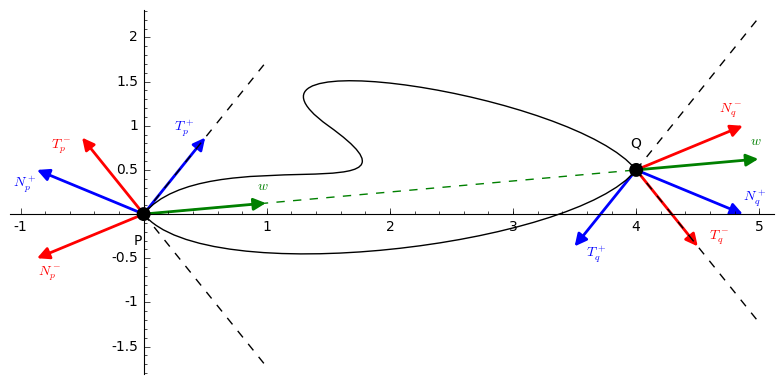
\includegraphics[width=.9\linewidth]{optimal_smooth}
\caption{The chord $\overline{p_0q_0} \subseteq \overline{\Omega}$ so that $w$ lies in the cones subtended by the dotted lines at $p_0$ and $q_0$.}
\label{fg:optimal_smooth}
\end{figure}

For equation \eqref{eq:optimal_regular_p}, noting that at \(p_0\), \(w\) is inward while \(\nor_{p_0}^+\) is outward, we write
\[
w = \cos \theta_{p_0}^+ \tang_{p_0}^+ - \sin \theta_{p_0}^+ \nor^+_{p_0}.
\]
The condition that \(w\) lies in the cone subtended by \(\tang_{p_0}^+\) and \(-\tang_{p_0}^-\) and the triple condition $\ip{\tang^+}{-\tang^-} = -\tfrac{1}{2} = \arccos\left(\tfrac{2\pi}{3}\right)$ (equation \eqref{eq:triplecondition}) implies that $0 \leq \theta^+_{p_0} \leq \tfrac{2\pi}{3}$. The triple conditions, equations \eqref{eq:triplecondition} and \eqref{eq:triplerelations} also imply that
\[
\tang_{p_0}^- = \frac{1}{2} \tang_{p_0}^+ + \tfrac{\sqrt{3}}{2} \nor_{p_0}^+
\]
Then,
\begin{equation}
\label{eq:optimal_regular_p_f}
\ip{\tang_{p_0}^- - \tang_{p_0}^+}{w} = - \left(\frac{1}{2} \cos \theta_{p_0}^+ + \frac{\sqrt{3}}{2} \sin \theta_{p_0}^+\right)
\end{equation}

Define,
\[
f(\theta) = \frac{1}{2} \cos \theta + \frac{\sqrt{3}}{2} \sin\theta
\]
Observe that,
\[
f(0) = f \left(\tfrac{2\pi}{3}\right) = \frac{1}{2},
\]
and on $[0, \tfrac{2\pi}{3}]$, $f$ is strictly concave. Thus $f > 0$ on $[0, \tfrac{2\pi}{3}]$, and hence by equation \eqref{eq:optimal_regular_p_f},
\[
\ip{\tang_{p_0}^- - \tang_{p_0}^+}{w} = - f (\theta_{p_0}^+) < 0
\]
proving equation \eqref{eq:optimal_regular_p}.

Equation \eqref{eq:optimal_regular_q} is similar noting that this time, at \(q_0\) both \(w\) and \(\nor_{q_0}^-\) are  outward pointing. Thus we write
\[
w = \cos \theta_{q_0}^- \tang_{p_0}^- + \sin \theta_{q_0}^- \nor^-_{q_0}
\]
again with $0 \leq \theta^-_{q_0} \leq \tfrac{2\pi}{3}$, and
\[
\tang_{q_0}^+ = \frac{1}{2} \tang_{q_0}^- - \tfrac{\sqrt{3}}{2} \nor_{q_0}^-.
\]
Hence,
\[
\ip{\tang_{q_0}^- - \tang_{q_0}^+}{w} = \left(\frac{1}{2} \cos \theta_{q_0}^- + \frac{\sqrt{3}}{2} \sin \theta_{q_0}^-\right) > 0
\]
proving equation \eqref{eq:optimal_regular_q}.
\end{proof}

As noted above, thanks to Lemma \ref{lem:optimum_are_regular}, we will only require the second variation at smooth points.

\begin{lemma}[Second Variation]
\label{lem:secondvar}
Let \((p,q)\) be a smooth point. Then,
\[
D^2 \ell = 0
\]
and
\[
\begin{split}
D^2d &= \left(\ip{w}{\curvecurv_p \nor_p} + \frac{1}{d}(1 - \ip{w}{\tang_p}^2) \right) \omega_p \tensor \omega_p \\
&+ \left(-\ip{w}{\curvecurv_q \nor_q} + \frac{1}{d}(1 - \ip{w}{\tang_q}^2) \right) \omega_q \tensor \omega_q \\
&- \left(\frac{1}{d}\left(\ip{\tang_p}{\tang_q} - \ip{w}{\tang_p}\ip{w}{\tang_q}\right) \right) \left(\omega_p \tensor \omega_q + \omega_q \tensor \omega_p\right).
\end{split}
\]
\end{lemma}

\begin{proof}
The second variation of \(\ell\) is immediate by differentiating the first variation in Lemma \ref{lem:firstvar}.

For the second variation of \(d\), we first differentiate $w$:
\[
\begin{split}
\partial_p w &= \partial_p \left[\frac{1}{d} (\gamma(q) - \gamma(p))\right] \\
&= \frac{1}{d^2} \ip{w}{\tang_p} (\gamma(q) - \gamma(p)) - \frac{1}{d} \tang_p \\
&= -\frac{1}{d}\left(\tang_p - \ip{w}{\tang_p} w\right).
\end{split}
\]
and similarly for $\pd{q} w$ (again with the sign changed).  Putting this together with the Frenet-Serret formula $\pd{p} \tang_p = -\curvecurv_p \nor_p$ \eqref{eq:frenetserret} then gives
\[
\begin{split}
\partial_p^2 d &= \partial_p \left[-\ip{\tang_p}{w}\right] \\
&= \ip{\frac{1}{d}\left(\tang_p - \ip{w}{\tang_p} w\right)}{\tang_p} + \ip{w}{\curvecurv_p \nor_p} \\
&= \frac{1}{d}\left(1 - \ip{w}{\tang_p}^2\right) + \ip{w}{\curvecurv_p \nor_p}.
\end{split}
\]
Similar computations give $\partial_q^2 d$. For the mixed partial,
\[
\begin{split}
\partial_q \partial_p d &= \partial_q \left[-\ip{w}{\tang_p}\right] \\
&= -\ip{\frac{1}{d}(\tang_q - \ip{\tang_q}{w}w)}{\tang_p} \\
&= - \frac{1}{d} \left(\ip{\tang_q}{\tang_p} - \ip{\tang_q}{w}\ip{\tang_p}{w}\right).
\end{split}
\]
These second derivatives yield the desired expression for \(D^2 d\).
\end{proof}

Using Lemmas \ref{lem:firstvar} and \ref{lem:secondvar} we may now obtain the second variation formula at smooth, optimal points. Let us first introduce some notation. Write \(\theta(p,q) \in (-\pi/2, \pi/2)\) for the angle between \(\tang_{p}\) and \(w\) so that \(\ip{w}{\tang_p} = \cos\theta\). Define the following "indicator" functions,
\begin{align*}
\tangindicator(p, q) &= \begin{cases}
1,& \tang_{p} \ne \tang_{q} \\
-1,& \tang_{p} = \tang_{q}
\end{cases} \\
\intertext{and}
\norindicator(p, q) &= \begin{cases}
1,& \ip{w}{\nor_{p}} > 0 \\
-1,& \ip{w}{\nor_{p}} < 0.
\end{cases}
\end{align*}
Define the bilinear forms,
\begin{align*}
K(p, q) &= \norindicator \left(\curvecurv_p \omega_p \otimes \omega_p + \tangindicator \curvecurv_q \omega_q \otimes \omega_q\right), \\
M(p, q) &= \omega_p \otimes \omega_p + \tangindicator\left(\omega_p \otimes \omega_q + \omega_q \otimes \omega_p\right) + \omega_q \otimes \omega_q.
\end{align*}
In matrix form, written with respect to the basis \(\{\tang_p, \tang_q\}\) we have,
\begin{align*}
K(p,q) &= \norindicator\begin{pmatrix}
\curvecurv_{p} & 0 \\
0 & \tangindicator \curvecurv_{q}
\end{pmatrix} \\
M(p,q) &= \begin{pmatrix}
1 & \tangindicator \\
\tangindicator & 1
\end{pmatrix}.
\end{align*}

Observe that \(M\) is diagonalised by the eigenvectors
\begin{equation}
\label{eq:eigenvectors}
v_1 = \tang_{p} + \tang_{q}, \quad v_2 = \tang_{p} - \tang_{q}
\end{equation}
with corresponding eigenvalues
\begin{equation}
\label{eq:eigenvalues}
\lambda_1 (p, q) = \begin{cases}
2, & \tangindicator = 1 \\
0, & \tangindicator = -1
\end{cases}
\quad
\lambda_2 (p, q) = \begin{cases}
0, & \tangindicator = 1 \\
2, & \tangindicator = -1
\end{cases}
\end{equation}

We express the variations of distance at an optimal point using this notation.

\begin{prop}[Spatial Variations At Smooth Optimal Points]
\label{prop:spatial_var}
Let $(p_0, q_0) \in \sphere^1 \times \sphere^1$ be smooth and optimal. Then
\[
\begin{split}
D d &= \cos\theta(-\omega_{p_0} + \omega_{q_0}) \\
\intertext{and}
D^2d_{(p_0,q_0)} &= \sqrt{1-\cos^2\theta}K + \frac{1-\cos^2 \theta}{d} M.
\end{split}
\]
\end{prop}

\begin{proof}
Consider the curve $\alpha: u \mapsto (p_0,q_0) + uv_1 = (p_0,q_0) + (u, u) \in \sphere^1\times \sphere^1$ which satisfies,
\[
\ell(\alpha(u)) = \ell(\alpha(0)).
\]
Thus $\ell$ is constant, equal to $\ell(p_0, q_0)$ along the curve $\alpha$.

Since $(p_0, q_0)$ minimises $d$ amongst all $(p,q)$ with $\ell(p, q) = \ell(p_0, q_0)$, we have that $u=0$ is a local minima of the function $u\mapsto d(\alpha(u))$. Then from the first variation of $d$ in Lemma \ref{lem:firstvar},
\[
0 = \left.\pd{u}\right|_{u=0} d(\alpha(u)) = -\ip{w}{\tang_{p_0}} + \ip{w}{\tang_{q_0}}
\]
so that
\[
\cos\theta = \ip{\tang_{p_0}}{w} = \ip{\tang_{q_0}}{w}
\]
yielding the desired first variation,
\[
Dd = \cos\theta(-\omega_{p_0} + \omega_{q_0}).
\]

We also have,
\[
\norindicator \sqrt{1 - \cos^2 \theta} = \ip{\nor_p}{w}
\]
recalling that \(\norindicator = \pm 1\) accordingly as \(w\) points outward or inward at \(p\).

Now, either $\tang_{p_0} = \tang_{q_0}$, or $\tang_{p_0} \ne \tang_{q_0}$ and $w$ bisects $\tang_{p_0}$ and $\tang_{q_0}$. These cases are recorded by the indicator function $\tangindicator$.

\emph{Case 1}: $\tang_{p_0} \ne \tang_{q_0}$ ($\tangindicator = 1$).

Assuming that $\tang_{p_0} \ne \tang_{q_0}$, since \(w\) bisects \(\tang_{p_0}\) and \(\tang_{q_0}\), we have
\[
-\ip{w}{\nor_{q_0}} = \ip{w}{\nor_{p_0}} = \norindicator \sqrt{1-\cos^2\theta}.
\]
Also since $w$ bisects $\tang_{p_0}$ and $\tang_{q_0}$, applying the double angle formula yields,
\[
\ip{\tang_{p_0}}{\tang_{q_0}} = 2\cos^2\theta - 1.
\]
Substituting these expressions into the second variation of $d$ from Lemma \ref{lem:secondvar} gives
\begin{align*}
D^2d_{(p_0,q_0)} &=  \left(\norindicator \sqrt{1-\cos^2\theta}\curvecurv_{p_0} + \frac{1}{d}(1 - \cos^2\theta) \right) \omega_{p_0} \tensor \omega_{p_0} \\
&+ \left(\norindicator \sqrt{1-\cos^2\theta} \curvecurv_{q_0} + \frac{1}{d}(1 - \cos^2\theta) \right) \omega_{q_0} \tensor \omega_{q_0} \\
&+ \left(\frac{1}{d}(1 - \cos^2\theta) \right) \left(\omega_{p_0} \tensor \omega_{q_0} + \omega_{q_0} \tensor \omega_{p_0} \right)
\end{align*}
which is the desired expression when $\tangindicator=1$.

\emph{Case 2}: $\tang_{p_0} = \tang_{q_0}$ ($\tangindicator = 1$).

In this case, we have 
\[
\ip{w}{\nor_{p_0}} = \ip{w}{\nor_{q_0}} = \norindicator \sqrt{1-\cos^2\theta}
\]
and $\ip{\tang_{p_0}}{\tang_{q_0}} = 1$. Substituting these expressions into the second variation of $d$  from Lemma \ref{lem:secondvar} gives
\begin{align*}
D^2d_{(p_0,q_0)} &=  \left(\norindicator \sqrt{1-\cos^2\theta}\curvecurv_{p_0} + \frac{1}{d}(1 - \cos^2\theta) \right) \omega_{p_0} \tensor \omega_{p_0} \\
&+ \left(-\norindicator \sqrt{1-\cos^2\theta} \curvecurv_{q_0} + \frac{1}{d}(1 - \cos^2\theta) \right) \omega_{q_0} \tensor \omega_{q_0} \\
&- \left(\frac{1}{d}(1 - \cos^2\theta) \right) \left(\omega_{p_0} \tensor \omega_{q_0} + \omega_{q_0} \tensor \omega_{p_0} \right)
\end{align*}
which gives the desired expression for $\tangindicator=1$ when expressed in matrix form.
\end{proof}

\subsection{Differential Inequalities}
\label{sec:orgheadline9}

In this section, using the variational formulae, we obtain a weak differential inequality for \(\chordarcprofile\). Theorem \ref{thm:barrier} is a barrier inequality, asserting the \emph{existence of a smooth, upper barrier} at regular points \(x_0\) (defined below). Such a barrier proves quite useful for deducing properties of the chord-arc profile in the sequel. As a corollary of the barrier inequality, we obtain Theorem \ref{thm:spatial_viscosity}, a viscosity equation for the chord-arc profile, asserting that \emph{if a smooth, lower support function exists}, it satisfies a certain differential inequality. The viscosity equation is weaker than the barrier inequality, and is not strictly necessary (one can work directly with the barrier inequality), but if provides a convenient formulation for comparisons.

Let us make the following definition.
\begin{defn}
The point \(x_0 \in (0, 2\pi)\) will be called a \emph{regular point} if there exists a smooth minimiser \((p_0, q_0)\). That is, if there exists \((p_0, q_0) \in \gamma^{\ast} \times \gamma^{\ast}\) such that \(\ell(p_0, q_0) = \tfrac{L}{2\pi} x_0\) and \(\chordarcprofile(x_0) = \tfrac{2\pi}{L} d(p_0, q_0)\).
\end{defn}

Our barrier inequality now reads as follows:

\begin{theorem}
\label{thm:barrier}
At regular points \(x_0\), the chord/arc-profile $\chordarcprofile$ satisfies the following differential inequality in the support (or barrier, or sometimes Calabi) sense
\begin{align*}
\chordarcprofile'_- &\leq \cos\theta \leq \chordarcprofile'_+, \\
\chordarcprofile'' &\leq \frac{L}{2\pi}\left[\frac{\norindicator \sqrt{1-\cos^2\theta}}{4} (\curvecurv_p + \tangindicator\curvecurv_q) + \frac{1}{2}(1-\tangindicator) \frac{1-\cos^2\theta}{d}\right].
\end{align*}
\end{theorem}

Recall that the support inequality means for every \(x_0 \in [0,2\pi]\) there exists a smooth, upper support function \(Z\) (\(Z(x) \geq \chordarcprofile (x)\), \(Z(x_0) = \chordarcprofile(x_0)\)) defined in a neighbourhood of \(x_0\) such that
\begin{align*}
Z' &= \cos \theta, \\
Z'' &= \frac{L}{2\pi}\left[\frac{\norindicator\sqrt{1-\cos^2\theta}}{4} (\curvecurv_p + \tangindicator\curvecurv_q) + \frac{1}{2} (1-\tangindicator) \frac{1-\cos^2\theta}{d}\right].
\end{align*}

\begin{proof}
For any $x_0$, let $(p_0,q_0)$ be such that $\ell(p_0,q_0) = \tfrac{L}{2\pi} x_0$ and $\chordarcprofile(x_0) = \tfrac{2\pi}{L} d(p_0,q_0)$. Consider the curve
\[
\alpha(u) = (p_0, q_0) + uv_2 = (p_0, q_0) + u(1,-1).
\]
Let \(x(u) = \tfrac{2\pi}{L} \ell(\alpha(u))\). We have
\[
\partial_u (\ell \circ \alpha) = -2
\]
so that $\ell\circ\alpha$ has a smooth local inverse near $u=0$: \(u = u(x) = (\ell \circ \alpha)^{-1}(\tfrac{L}{2\pi} x)\) satisfying \(u(x_0) = 0\) and \(u'(x) = -\tfrac{L}{4\pi}\).

Define
\[
Z(x) = \frac{2\pi}{L} d(\alpha \circ u (x))
\]
which is indeed a smooth, upper support function, since
\begin{align*}
Z(x_0) &= \frac{2\pi}{L} d(\alpha(0)) = \frac{2\pi}{L} d(p_0, q_0) = \chordarcprofile(x_0) \\
\intertext{and}
Z(x) &= \frac{2\pi}{L} d(\alpha \circ u(x)) \geq \chordarcprofile \left(\frac{2\pi}{L}\ell\circ\alpha(u(x))\right) = \chordarcprofile(x).
\end{align*}

Observe that $\alpha' = v_2 = \tang_{p_0} - \tang_{q_0}$ so that \(\partial_x \alpha(u(x)) = -\tfrac{L}{4\pi} v_2\). Using also the first variation of $d$ at optimal points in Proposition \ref{prop:spatial_var}
\[
Z'(x_0) = \frac{2\pi}{L} Dd \cdot \left(-\frac{L}{4\pi}v_2\right) = -\frac{1}{2} \cos\theta (-\omega_{p_0} + \omega_{q_0}) \cdot (\tang_{p_0} - \tang_{q_0}) = \cos\theta
\]
proving the first equation.

For the second equation, we have
\[
Z''(x_0) = \frac{2\pi}{L} D^2 d \left(-\frac{L}{4\pi} v_2, -\frac{L}{4\pi} v_2\right) = \frac{L}{8\pi} D^2 d (v_2, v_2)
\]
as a bilinear form. Now apply Proposition \ref{prop:spatial_var} to obtain
\begin{equation}
\label{eq:barrier_secondvar}
Z''(x_0) = \frac{L}{8\pi} \left(\sqrt{1-\cos^2\theta} K (v_2, v_2) + \frac{1-\cos^2\theta}{d} M (v_2, v_2)\right).
\end{equation}

We have,
\[
K(v_2, v_2) =
\begin{pmatrix}
1 & -1
\end{pmatrix}
\begin{pmatrix}
\curvecurv_{p} & 0 \\
0 & \tangindicator \curvecurv_{q}
\end{pmatrix}
\begin{pmatrix}
1 \\
-1
\end{pmatrix}
= \curvecurv_p + \tangindicator \curvecurv_q
\]
and
\[
M(v_2, v_2) = \begin{pmatrix}
1 & -1
\end{pmatrix}
\begin{pmatrix}
1 & \tangindicator \\
\tangindicator & 1
\end{pmatrix}
\begin{pmatrix}
1 \\
-1
\end{pmatrix}
= \begin{cases}
0, & \tangindicator = 1 \\
4, & \tangindicator = -1.
\end{cases}
\]

Substitution in equation \eqref{eq:barrier_secondvar} gives the desired expression.
\end{proof}

\begin{remark}
In the case \(\tangindicator = 1\), the second term of \(\chordarcprofile''\) is not present. This is because \(v_2\) is an eigenvector of \(M\) with eigenvalue \(\lambda_2 = 0\) in the case \(\tangindicator = 1\). In the case \(\tangindicator = -1\), the corresponding eigenvalue is \(\lambda_2 = 2\) and so the second term is not annihilated. We might like to try annihilate this term by using \(v_1\) instead of \(v_2\) in the case \(\tangindicator = -1\), but this leads to the vacuous equation \(0 = 0\) since the corresponding curve \(\alpha(u) = (p_0, q_0) + u v_1\) preserves length.
\end{remark}

We finish this section with the viscosity equation.

\begin{theorem}
\label{thm:spatial_viscosity}
At a regular point \(x_0\), the chord-arc profile $\chordarcprofile$ of \(\gamma\) satisfies the following inequality in the viscosity-sense:
\[
-\frac{\chordarcprofile''}{\sqrt{1-(\chordarcprofile')^2}} + \frac{1}{2} (1-\tangindicator) \frac{\sqrt{1 - (\chordarcprofile')^2}}{\chordarcprofile} \geq -\frac{L}{8\pi} \norindicator \left[\curvecurv_p + \tangindicator \curvecurv_q\right].
\]
\end{theorem}

This means that for any regular point \(x_0 \in (0,2\pi)\), if \(\varphi\) is a local, smooth, lower supporting function at \(x_0\), (\(\varphi\) is defined in a neighbourhood of \(x_0\) and \(\varphi(x) \leq \chordarcprofile (x)\), \(\varphi(x_0) = \chordarcprofile (x_0)\)), then \(\varphi\) satisfies the inequality in the usual sense. The coefficients, \(\tangindicator, \norindicator, \curvecurv_p, \curvecurv_q\) are evaluated at an optimal point \((p_0, q_0)\) for \(x_0\) and though determined, are a priori unknown.

\begin{proof}
Fix a regular point, $x_0 \in (0,2\pi)$ and suppose $\varphi(x)$ is a smooth function defined in neighbourhood of $x_0$ such that $\varphi(x_0) = \chordarcprofile(x_0)$ and $\varphi(x) \leq \chordarcprofile(x)$. Let \(Z\) denote the smooth, upper barrier function constructed in Theorem \ref{thm:barrier} at \(x_0\). Then,
\[
Z(x) - \varphi(x) \geq \chordarcprofile(x) - \varphi(x) \geq 0, \quad Z(x_0) - \varphi(x_0) = \chordarcprofile(x_0) - \chordarcprofile(x_0) = 0.
\]
Thus the smooth function \(Z(x) - \varphi(x)\) has a local minimum at \(x_0\), hence
\[
Z'(x_0) = \varphi'(x_0), \quad Z''(x_0) \geq \varphi''(x_0).
\]
We also have,
\[
\varphi(x_0) = \chordarcprofile(x_0) = \frac{2\pi}{L} d(p_0, q_0)
\]
where \((p_0, q_0)\) is optimal for \(x_0\).

Recall, Theorem \ref{thm:barrier} implies
\begin{align*}
Z'(x_0) &= \cos \theta, \\
Z''(x_0) &= \frac{L}{2\pi}\left[\frac{\norindicator\sqrt{1-\cos^2\theta}}{4} (\curvecurv_p + \tangindicator\curvecurv_q) + \frac{1}{2} (1-\tangindicator) \frac{1-\cos^2\theta}{d}\right].
\end{align*}

Thus \(\varphi' = \cos \theta\) and,
\[
\varphi'' \leq \frac{L}{2\pi}\left[\frac{\norindicator\sqrt{1-(\varphi')^2}}{4} (\curvecurv_p + \tangindicator\curvecurv_q) + \frac{1}{2} (1-\tangindicator) \frac{1-(\varphi')^2}{\tfrac{L}{2\pi} \varphi}\right].
\]
Rearranging gives the proof.
\end{proof}

\section{Convex Networks}

We now consider the implications of the variational formulae and differential inequalities in the case of convex networks. These are rather more well behaved than general networks, and serve as a model case. In particular, the chord-arc profile is concave. We also deduce some properties for general networks at optimal points that behave similar to the convex case, in particular relating local concavity of the profile to convex-like behaviour at corresponding optimal points. The analysis, particularly of the second variation affords control of the topology of optimal points (through the indicator functions) essential to the comparison arguments later.

\begin{remark}
First let us remark that convex networks are constrained in the maximum number of nodes possible. In the proof of Lemma \ref{lem:dtA}, we used,
\[
\int \curvecurv ds = (2 - \frac{k}{3}) \pi.
\]
From this equation we may also conclude that if \(\gamma\) is a convex network (so that \(\curvecurv \geq 0\)) with \(k\) nodes satisfying the triple condition \eqref{eq:triplecondition}, then \(k \leq 6\). In the case \(k = 6\), we must have \(\curvecurv \equiv 0\) so that \(\gamma\) is an equi-angular hexagon, and either this condition must be preserved by the network curve shortening flow, or convexity must be lost. What happens is determined by the unbounded curves \(L_i\). In particular, if all the \(L_i\) are straight lines, then such a network is a static solution. Otherwise, we expect the curvature of the \(L_i\) to drive the loop away from convexity. Notice that to keep the loop static, the unbounded curves would need to satisfy the curve shortening flow along with fixed boundary conditions (as the node is stationary) and fixed gradient at the boundary (as the angle must be preserved). This is an over-determined system so we do not expect the loop to be static if at least one of the \(L_i\) is not a straight line.
\end{remark}

Convex networks are very nice in that all optimal points are smooth.

\begin{lemma}
\label{lem:convex_regular}

Let \(\gamma\) be convex and \((p_0,q_0) \in \sphere^1 \times \sphere^1\) be optimal. Then \((p_0, q_0) \in \gamma^{\ast} \times \gamma^{\ast}\).
\end{lemma}

\begin{proof}
If $\gamma$ is convex, then $\overline{\Omega}$ is a closed convex set with $\gamma(p_0), \gamma(q_0) \in \overline{\Omega}$ whence the chord $\overline{p_0q_0} \subseteq \overline{\Omega}$ and Lemma \ref{lem:optimum_are_regular} applies.
\end{proof}

More generally, as simlar argument allows us to exploit concavity properties of the chord/arc-profile. In particular, it shows that if the chord-arc profile is supported from below by a concave function (``concavity at a point''), then the corresponding optimal points are convex-like.

\begin{lemma}
\label{lem:concave_barrier}
If there exists a strictly concave, positive function $\phi: (0, 2\pi) \to \RR$ that is symmetric about $\pi$ and supporting $\chordarcprofile$ at $x_0=\tfrac{2\pi}{L} \ell(p_0,q_0)$ from below (so that $\phi(x) \leq \chordarcprofile(x)$ and $\phi(x_0)=\chordarcprofile(x_0)$), then $x_0$ is regular, $\tangindicator = 1$, and $\norindicator = 1$.
\end{lemma}

\begin{proof}
We proceed similarly to \cite{MR2794630} by showing that $\overline{p_0q_0} \subseteq \overline{\Omega}$. Suppose then that there is a $\phi$ as in the statement of the lemma, and in order to obtain a contradiction, that $\overline{p_0q_0}$ is not contained in $\overline{\Omega}$. Thus there is a point $s$ such that $\overline{p_0q_0}$ intersects $\gamma$ at $s$. We may assume that an intersection occurs at $s$ with $p_0 < s < q_0$. Then we have
\begin{align*}
d(p_0, q_0) &= d(p_0, s) + d(s, q_0) \\
\ell(p_0, q_0) &= \min\{\ell(p_0, s) + \ell(s, q_0),  2\pi -\ell(p_0,s ) - \ell(s, q_0)\}.
\end{align*}
Since $\phi$ is strictly concave, $\phi(x + y) = \phi(x + y) + \phi(0) \leq \phi(x) + \phi(y)$ whenever $x, y > 0$ and $x + y < 2\pi$. Noting also that $\phi(x) = \phi(2\pi - x)$, we have
\[
\begin{split}
0 &= \chordarcprofile(\ell(p_0, q_0)) - \phi(\ell(p_0, q_0)) \\
&=  d(p_0, q_0) - \phi(\ell(p_0, q_0)) \\
&= d(p_0, s) + d(s, q_0) - \phi(\ell(p_0, s) + \ell(s,  q_0)) \\
&> d(p_0, s) - \phi(\ell(p_0, s)) + d(s, q_0) - \phi(\ell(s, q_0)) \\
&\geq \chordarcprofile(\ell(p_0, s)) - \phi(\ell(p_0, s)) + \chordarcprofile(\ell(s, q_0)) - \phi(\ell(s, q_0)) \\
&\geq 0.
\end{split}
\]
Thus we have our contradiction. Therefore $\overline{p_0q_0} \subseteq \overline{\Omega}$ and by Lemma \ref{lem:optimum_are_regular}, \(x_0\) is regular. Morevoer, since $w$ points inward, $\norindicator = 1$.

To show that $\tangindicator = 1$, suppose that $\tang_{p_0} = \tang_{q_0}$. Then the normal makes an acute angle with the chord $\overline{p_0 q_0}$ at one endpoint, and an obtuse angle at the other. Therefore points on the chord $\overline{p_0q_0}$ near one endpoint are inside $\Omega$, while points near the other endpoint are outside contradicting $\overline{p_0q_0} \subset \overline{\Omega}$.
\end{proof}

Finally, let us note an important property of convex networks.

\begin{theorem}
\label{thm:convex_network_concave_profile}

If $\gamma$ is convex, then $\chordarcprofile$ is concave and if $\gamma$ is strictly convex, then $\chordarcprofile$ is strictly concave.
\end{theorem}

\begin{proof}
If $\gamma$ is convex, then by lemma \ref{lem:convex_regular} all points $x \in (0, 2\pi)$ are regular. Moreover, $\curvecurv \geq 0$ and $\tang_{p_0} \ne \tang_{q_0}$ so that $\xi = 1$, while \(w\) points inward at $p_0$ as in lemma \ref{lem:convex_regular} ensuring that $\delta = 1$. Therefore, at every point $x$, the upper barrier $Z$ from Theorem \ref{thm:barrier} satisfies
\[
Z'' \leq - \frac{\sqrt{1-\cos^2 \theta}}{4} (\curvecurv_{p_0} + \curvecurv_{q_0}) \leq 0.
\]
Thus $\chordarcprofile$ is supported above by a concave function at all points. Hence $\chordarcprofile$ is itself concave \cite[Lemma 2.7]{MR1674097}.
\end{proof}

\begin{remark}
Compare the above with similar results obtained in \cite{MR1674097}, pertaining to isoperimetric regions of convex bodies in Euclidean space and in \cite{MR875084}, pertaining to isoperimetric regions in compact surfaces. As described in \cite{pbthesis}, both arguments lead to the concavity of $\isoprofile^2(x) + K_0 x^2$ where $\isoprofile$ is the isoperimetric profile, and $K_0$ is a lower bound on boundary mean curvature or ambient Gauss curvature respectively. In particular, if the curvature is non-negative, then not only is the isoperimetric profile concave, but it's square also. Here, the analogous result is not true for the chord/arc-profile in the strongest possible sense as seen by the simple counter-example of the unit circle, whose chord/arc-profile is
\[
\chordarcprofile_{\sphere^1} (x) = 2 \sin \left(\frac{x}{2}\right).
\]
This is a strictly concave function whose square is not concave. This seems related to the fact that the local behaviour of the chord/arc-profile is determined by the \emph{square} of the curvature, $\curvecurv^2$ as opposed to the isoperimetric profile of a surface or convex body in the plane, which is locally determined by the curvature (Gauss curvature for compact surfaces and boundary mean curvature for convex bodies in Euclidean space).
\end{remark}

\section{Viscosity Equation For Networks Evolving By Curve Shortening}
\label{sec:viscosity_csf}

Now we may prove the theorem at the heart of our method. First, let us define,
\begin{equation}
\label{eq:Q}
\bar{Q} = \int_{\gamma} \curvecurv^2 ds - \frac{1}{\sqrt{3}} \sum_{m=1}^{k} \curvecurv_m^+ + \curvecurv_m^-
\end{equation}
and
\begin{equation}
\label{eq:delQ}
\Delta Q(p_0, q_0) = \int_p^q \curvecurv^2 ds - \sum_{m=i}^{j-1} \curvecurv_m^+ + \curvecurv_m^-
\end{equation}

Then Lemma \ref{lem:distance_evolution} may be rewritten,
\begin{equation}
\label{eq:distance_evolution_q}
\begin{split}
\partial_t d_t(p, q) &= -\curvecurv_q \ip{\nor_q}{w} + \curvecurv_p \ip{\nor_p}{w} + \tangspeed_q \ip{\tang_q}{w} - \tangspeed_p \ip{\tang_p}{w}, \\
\partial_t \ell_t(p, q) &= -\Delta Q(p_0, q_0) + \tangspeed_{q_0} - \tangspeed_{p_0} \\
\partial_t L &= -\bar{Q}
\end{split}
\end{equation}

\begin{theorem}
\label{thm:csf_viscosity}

Let $\gamma$ be the loop of a network evolving by the Curve Shortening Flow. Then at regular points, the Chord-Arc profile $\gamma$ satisfies the following viscosity equation
\[
\partial_t \chordarcprofile \geq \left(\frac{2\pi}{L}\right)^2 \left(4 \chordarcprofile'' - 2 (1-\tangindicator) \frac{1 - (\chordarcprofile')^2}{\chordarcprofile}\right) + \left(\chordarcprofile - x \chordarcprofile'\right) \frac{1}{L} \bar{Q} + \frac{2\pi}{L} \chordarcprofile' \Delta Q.
\]
\end{theorem}

\begin{proof}
For the parabolic version of viscosity equation we need to prove that for any $(x_0, t_0) \in (0, 2\pi) \times [0, T)$ and any smooth, lower supporting function $\phi$ defined on $(x_0 -\epsilon, x_0 + \epsilon) \times (t_0 - \epsilon, t_0]$ (for some $\epsilon > 0$) then $\phi$ satisfies the differential inequality of the theorem.

Suppose then that such a $\phi$ exists and let $(p_0, q_0)$ be an optimal, smooth point for the $\gamma_{t_0}$. Then we have
\[
\frac{2\pi}{L} d(p_0, q_0, t_0) = \chordarcprofile\left(\frac{2\pi}{L} \ell(p_0, q_0, t_0)\right) = \phi\left(\frac{2\pi}{L} \ell(p_0, q_0, t_0), t\right)
\]
and
\[
\frac{2\pi}{L} d(p_0, q_0, t) \geq \chordarcprofile\left(\frac{2\pi}{L} \ell(p_0, q_0, t)\right) \geq \phi\left(\frac{2\pi}{L} \ell(p_0, q_0, t), t\right)
\]
for $t \leq t_0$. Therefore,
\[
- \frac{2\pi d}{L} \frac{\partial_t L}{L} + \frac{2\pi}{L} \partial_t d \leq \partial_t \phi - \phi' \frac{2\pi \ell}{L} \frac{\partial_t L}{L} +\phi' \frac{2\pi}{L} \partial_t l.
\]

Substituting \eqref{eq:distance_evolution_q} gives,
\begin{equation}
\label{eq:time_ineq}
\begin{split}
\partial_t \phi &\geq \frac{2\pi}{L} \left[-\curvecurv_{q_0} \ip{\nor_{q_0}}{w} + \curvecurv_{p_0} \ip{\nor_{p_0}}{w} + \tangspeed_{q_0} \ip{\tang_{q_0}}{w} - \tangspeed_{p_0} \ip{\tang_{p_0}}{w}\right] \\
&\quad + \left(\frac{2\pi d}{L} - \phi' \frac{2\pi \ell}{L}\right) \frac{1}{L} \bar{Q} + \frac{2\pi}{L} \phi' \Delta Q \\
&\quad - \frac{2\pi}{L} \phi' \left(\tangspeed_{q_0} - \tangspeed_{p_0}\right) \\
&= \frac{2\pi}{L} \left[-\curvecurv_{q_0} \ip{\nor_{q_0}}{w} + \curvecurv_{p_0} \ip{\nor_{p_0}}{w}\right] + \left(\phi - x \phi'\right) \frac{1}{L} \bar{Q} + \frac{2\pi}{L} \phi' \Delta Q
\end{split}
\end{equation}
where we applied Theorem \ref{thm:barrier} giving $\phi' = \ip{\tang_{q_0}}{w} = \ip{\tang_{p_0}}{w}$.

On the other hand, at $t_0$, $x \mapsto \phi(x, t_0)$ is a lower supporting function for $x \mapsto \chordarcprofile(x, t_0)$ and hence,
\begin{equation}
\label{eq:spatial_inequality}
-\frac{\phi''}{\sqrt{1-(\phi')^2}} + \frac{1}{2} (1-\tangindicator) \frac{\sqrt{1 - (\phi')^2}}{\phi} \geq -\frac{L}{8\pi} \norindicator \left[\curvecurv_p + \tangindicator \curvecurv_q\right]
\end{equation}
by the spatial viscosity equation Theorem \ref{thm:spatial_viscosity} at regular points. Recalling that,
\[
\norindicator \sqrt{1 - (\phi')^2} \left[\curvecurv_p + \tangindicator \curvecurv_q\right] = \left[\curvecurv_{p_0} \ip{\nor_{p_0}}{w} - \curvecurv_{q_0} \ip{\nor_{q_0}}{w}\right]
\]
and combining with \eqref{eq:time_ineq}, we get
\[
\partial_t \phi \geq \left(\frac{2\pi}{L}\right)^2 \left(4 \phi'' - 2 (1-\tangindicator) \frac{1 - (\phi')^2}{\phi}\right) + \left(\phi - x \phi'\right) \frac{1}{L} \bar{Q} + \frac{2\pi}{L} \phi' \Delta Q.
\]
\end{proof}

We may now deduce the comparison theorem. For this we also make a normalisation of the time variable.

\begin{theorem}
\label{thm:comparison}

Let $\varphi_0 : [0, 2\pi] \times \RR_{\geq 0} \to \RR$ be a continuous function satisfying:
\begin{itemize}
\item $\varphi_0$ is smooth and positive on $(0, 2\pi) \times \RR_{>0}$,
\item $\varphi_0(\cdot, \tau)$ is symmetric about $x = \pi$ for every $\tau$,
\item $\varphi_0(0, \tau) = \varphi_0(2\pi, \tau) = 0$ for every $\tau$,
\item $\varphi_0$ is weakly concave in $x$ for each $\tau$ ($\varphi_0'' \leq 0)$,
\end{itemize}
and such that
\begin{equation}
\label{eq:comparison_ineq}
\partial_{\tau} \varphi_0 \leq 4 \varphi_0'' + \frac{L}{4\pi^2} \bar{Q} (\varphi_0 - x \varphi_0') + \frac{L}{2\pi} \Delta Q \varphi_0'.
\end{equation}
If $\varphi_0(x, 0) \leq \chordarcprofile(x, 0)$ for all $x \in [0, 2\pi]$, then $\varphi(x, t) := \varphi_0(x, \tau(t)) \leq \chordarcprofile(x, t)$ for all $x, t$ where $\tau$ satisfies
\[
\begin{cases}
\partial_t \tau &= \left(\frac{2\pi}{L}\right)^2 \\
\tau(0) &= 0.
\end{cases}
\]

If in addition,
\[
\varphi_0(x, \tau) = \frac{\sqrt{3}}{2} x - c(\tau) x^2 + \bigo(x^3) \quad \text{as} \quad x \to 0
\]
then
\[
\frac{L}{2\pi} \max_i \{\curvecurv^+(a_i, t) + \curvecurv^-(a_i, t)\} \leq 16 c(\tau(t)).
\]
for all $t$.
\end{theorem}

\begin{remark}
Note that the coefficients $\tfrac{L}{4\pi^2} \bar{Q}$ and $\tfrac{L}{2\pi}\Delta Q$ are scale invariant. Without the change of time parameter $\tau$, we would not obtain a scale invariant equation. The change in time precisely compensates for the lack of uniform time interval among solutions of the flow, providing the desired scale invariant equation.
\end{remark}

\begin{proof}
Let $\varphi(x, t) = \varphi_0(x, \tau(t))$. The assumptions on $\varphi_0$ give
\[
\partial_t \varphi = \left(\frac{2\pi}{L}\right)^2 \partial_{\tau} \varphi_0 \leq 4 \left(\frac{2\pi}{L}\right)^2 \varphi_0'' + \left(\frac{2\pi}{L}\right)^2 \frac{L}{4\pi^2} \bar{Q} (\varphi_0 - x \varphi_0') + \left(\frac{2\pi}{L}\right)^2 \frac{L}{2\pi} \Delta Q \varphi_0'.
\]
For convenience, define
\[
F(z, p, y, x, t) = \left(\frac{2\pi}{L}\right)^2 4 z + \frac{1}{L} \bar{Q} (y - x p) + \frac{2\pi}{L} \Delta Q p.
\]
so that $\varphi$ satisfies,
\begin{equation}
\label{eq:comparison_diff_ineq_leq}
\partial_t \varphi \leq F(\varphi'', \varphi', \varphi, x, t).
\end{equation}

Owing to a lack of suitable monotonicity of $F$ in the $y$ variable, we must introduce an exponential factor. We first claim that for any $\lambda > 0$, at regular points, the function $e^{-\lambda t} \chordarcprofile$ is a viscosity solution of
\begin{equation}
\label{eq:exponential_viscosity}
\partial_t \chordarcprofile \geq e^{-\lambda t} F_{\lambda} (e^{\lambda t} \chordarcprofile'', e^{\lambda t} \chordarcprofile', e^{\lambda t} \chordarcprofile, x, t) - \left(\frac{2\pi}{L}\right)^2 2 (1-\tangindicator) \frac{1 - (e^{\lambda t} \chordarcprofile')^2}{e^{2\lambda t} \chordarcprofile}
\end{equation}
where
\[
F_{\lambda}(z, p, y, x, t) = F(z, p, y, x, t) - \lambda y.
\]
To see this, note if $\psi \leq e^{-\lambda t} \chordarcprofile$ for $t\leq t_0$ with equality at $(x_0, t_0)$, then $e^{\lambda t} \psi \leq \chordarcprofile$ for $t\leq t_0$ with equality at $(x_0, t_0)$. Therefore the viscosity equation for $\chordarcprofile$ in Theorem \ref{thm:csf_viscosity} gives
\[
e^{\lambda t} (\partial_t \psi + \lambda \psi) = \partial_t (e^{\lambda t} \psi) \geq F(e^{\lambda t} \psi'', e^{\lambda t} \psi', e^{\lambda t} \psi, x, t) - \left(\frac{2\pi}{L}\right)^2 2 (1-\tangindicator) \frac{1 - (e^{\lambda t} \chordarcprofile')^2}{e^{\lambda t} \chordarcprofile}
\]
at $(x_0, t_0)$, and so
\[
\begin{split}
\partial_t \psi &\geq e^{-\lambda t} F(e^{\lambda t} \psi'', e^{\lambda t} \psi', e^{\lambda t} \psi, x, t) - \lambda \psi - \left(\frac{2\pi}{L}\right)^2 2 (1-\tangindicator) \frac{1 - (e^{\lambda t} \chordarcprofile')^2}{e^{2\lambda t} \chordarcprofile} \\
&= e^{-\lambda t} \left[F(e^{\lambda t} \psi'', e^{\lambda t} \psi', e^{\lambda t} \psi, x, t) - \lambda e^{\lambda t} \psi\right] - \left(\frac{2\pi}{L}\right)^2 2 (1-\tangindicator) \frac{1 - (e^{\lambda t} \chordarcprofile')^2}{e^{2\lambda t} \chordarcprofile} \\
&= e^{-\lambda t} F_{\lambda}(e^{\lambda t} \psi'', e^{\lambda t} \psi', e^{\lambda t} \psi, x, t) - \left(\frac{2\pi}{L}\right)^2 2 (1-\tangindicator) \frac{1 - (e^{\lambda t} \chordarcprofile')^2}{e^{2\lambda t} \chordarcprofile}
\end{split}
\]
at $(x_0, t_0)$ as claimed.

Now suppose the theorem is false. Then there must be a $\tau \in (0, T)$ such that
\[
\inf_{(x, t) \in [0, 2\pi] \times [0,\tau]} \{\chordarcprofile(x, t) - \varphi(x, t)\}  < 0.
\]
Then letting
\[
m = -\inf_{(x, t) \in [0, 2\pi] \times [0,\tau]} \{e^{-\lambda t} \chordarcprofile(x, t) - e^{-\lambda t} \varphi(x, t)\}
\]
we have $m > 0$. By compactness we may choose $(x_0, t_0)$ such that $e^{-\lambda t_0} \chordarcprofile(x_0, t_0) - e^{-\lambda t_0} \varphi(x_0, t_0) = -m$. Define
\[
\psi = e^{-\lambda t} \varphi - m
\]
which is then a lower support function for $e^{-\lambda t} \chordarcprofile$ at $(x_0, t_0)$. Then also $\varphi - m e^{\lambda t_0}$ is a concave, lower supporting function for $\chordarcprofile$ at $(x_0, t_0)$, hence Lemma \ref{lem:concave_barrier} ensures that $\tangindicator = 1$ and that $x_0$ is a regular point of $\chordarcprofile(\cdot, t_0)$. The viscosity equation \eqref{eq:exponential_viscosity} for $e^{-\lambda t}\chordarcprofile$ then gives,
\[
\partial_t \psi \geq e^{-\lambda t} F_{\lambda} (e^{\lambda t} \psi'', e^{\lambda t} \psi', e^{\lambda t} \psi, x, t) = e^{-\lambda t} F_{\lambda} (\varphi'', \varphi', \varphi - m e^{\lambda t}, x, t)
\]

On the other hand, the assumed inequality \eqref{eq:comparison_diff_ineq_leq} for $\varphi$ gives,
\[
\partial_t \psi = e^{-\lambda t} (\partial_t \varphi - \lambda \varphi) \leq e^{-\lambda_t}(F(\varphi'', \varphi', \varphi, x, t)  - \lambda \varphi) = e^{-\lambda t} F_{\lambda}(\varphi'', \varphi', \varphi, x, t)
\]

Putting the two previous inequalities together then yields
\begin{equation}
\label{eq:F_leq}
F_{\lambda} (\varphi'', \varphi', \varphi - m e^{\lambda t}, x, t) \leq F_{\lambda}(\varphi'', \varphi', \varphi, x, t)
\end{equation}

But now, from the definition of $F$ we have
\[
F_{\lambda} (z, p, y, x, t) = \left(\frac{2\pi}{L}\right)^2 4 z + (\frac{1}{L} \bar{Q} - \lambda) y - \frac{1}{L} \bar{Q} x p + \frac{2\pi}{L} \Delta Q p.
\]
Choosing
\[
\lambda > \sup_{(x, t) \in [0, 2\pi] \times [0, \tau]} \frac{1}{L} \bar{Q},
\]
makes $F_{\lambda}$ strictly decreasing in the $y$ variable and hence
\[
F_{\lambda} (\varphi'', \varphi', \varphi - m e^{\lambda t}, x, t) > F_{\lambda}(\varphi'', \varphi', \varphi, x, t)
\]
since $\varphi - m e^{\lambda t} < \varphi$. Thus we have a contradiction to \eqref{eq:F_leq} proving the first part of the theorem.

For the second part, recall Proposition \ref{prop:asymptotics} states that
\[
\chordarcprofile(x, t) = \frac{\sqrt{3}}{2}x - \frac{L}{32\pi} \max_i \{\curvecurv^+(a_i) + \curvecurv^-(a_i)\} x^2 + \bigo(x^3) \quad \text{as} \quad x \to 0.
\]
Hence the assumed asymptotic behaviour of $\varphi$ along with the inequality $\varphi(x, t) \leq \chordarcprofile(x, t)$ yields the second part.
\end{proof}

\section{Self-similar Profiles}

In this section we describe the profile for self similar solutions on the skeletons fixed in Section \ref{sec:self_similar}. Note that to cover half of the length of the network we need to cross $\frac{n}{2}$ nodes. At those points the profile will be continuous, but not differentiable.

We start by giving a more accurate description of the self-similar profile $\sqrt{1-st}\gamma_0(x)$ at time $t=\frac{1}{2}$. We assume that $\gamma_0$ is parametrized according to its arc-length, then the equation satisfied by $\gamma_0$ is
\begin{equation} -\gamma_0= v \tang- \curvecurv \nor= v \gamma_0'+\gamma_0''.
\label{eq:self-similar curve}
\end{equation}

From this equation we have that
$$v=- \ip{\gamma_0}{\gamma_0'}.$$
Equivalently,

$$v'=-1+\curvecurv\ip{\gamma_0}{\nor} =-1+\curvecurv^2.$$
Integrating this expression between $p_0$ and $q_0$ we obtain

\begin{align*}
v(q_0)-v(p_0)=& - l+\Delta Q_0,\\
\bar{Q}_0=&L_0,
\end{align*}
where $L_0$ is the length of the given self-similar solutions.

Some further remarks about the self-similar solution:

\begin{enumerate}
\item The enclosed area is given
$$\area=\frac{1}{2}\int \ip{\gamma}{\nor}=\frac{1}{2}\int \curvecurv=\frac{1}{2}\left(2\pi-\frac{k}{3}\right).$$
\item If this curve minimizes length for that given area, it should compare with a piece of a circle satisfying the correct angular condition (I am not sure how to argue this yet). Not sure this bound is useful in anyway.
\end{enumerate}


We fix a vector $v$ and show that $\psi_0(x)=2\ip{\gamma_0\left(\frac{x}{2}\right)}{v}$ satisfies the equation for chord-arc profiles:

\begin{align*}
\psi_0'= &\ip{\gamma_0'\left(\frac{x}{2}\right)}{v},\\
\psi_0''= &\frac{1}{2}\ip{\gamma_0''\left(\frac{x}{2}\right)}{v}.
\end{align*}
We also note that these curves are convex, hence $\tangindicator=1$.

From Equation \eqref{eq:self-similar curve} we have
$$4\psi_0''=-\psi_0-2v\left(\frac{x}{2}\right) \psi_0'. $$
Using the definition of $v$ we have
$$4\psi_0''=-\psi_0-\left(2\frac{x}{2}-2\Delta Q(\frac{x}{2})\right) \psi_0'. $$

Recalling that $\bar{Q}{L}=1$ and the symmetry we have the desired equation. 


The vector $v$ is chosen such that the boundary condition is met at $x=0$.

{\color{red} need to describe how we pass through nodes and when it jumps, but is should be when we go through half of each curve. Note that if we are jumping 2 nodes (and have at most 5 sides, then jumping 3 nodes is like jumping 2 on the other side (so there should be more symmetries. }

We do it carefully for $n=2,3,4,5, 6$ faces (we need to check if this idea works in the expanding case)

For a self-similar solution solution, \(\sigma\), let us write \(\psi\) for the chord arc-profile of \(\sigma\).

\begin{lemma}
Let \(\gamma_0\) be a self-similar solution with chord-arc profile $\psi_0$. Then there exists a convex function $f_0$ such that
\[
\tfrac{L}{2\pi} \Delta Q_0 (x) = \frac{1}{x} f_0(\psi_0'(x)).
\]
\end{lemma}

\begin{proof}

\end{proof}

\section{Comparison Functions}
\label{sec:orgheadline11}

In this section, we seek suitable functions $\varphi_0$ satisfying the hypotheses of Theorem \ref{thm:comparison}. Our approach is to seek a one-parameter family $\varphi_c$ of such functions such that for any given curve there is a $c$ with $\varphi_c(x, 0) \leq \chordarcprofile(x, 0)$. Such functions are constructed as in \cite{MR2794630} by making a change of variables $x \mapsto \psi_0(x)$ where $\psi_0(x)$ is the profile of a self-similar solution to the flow while simultaneously changing the time parameter $\tau \mapsto e^{\tau}$. Then we seek a similarity solution of the resulting ODE. That is we make the ansatz,
\[
\varphi_0(x, \tau) = e^{\tau} \Phi(e^{-\tau} \psi_0(x)).
\]

\begin{theorem}
\label{thm:comparison_function}
Let
\[
\Phi_c(u) = 
\]
and
\[
\varphi_c(x, \tau) = e^{\tau} \Phi_c(e^{-\tau} \psi_0(x))
\]
with $\psi_0$ a self-similar solution of the Network CSF with a single loop and $k$ nodes.

Let $\gamma$ be a a solution of the network CSF such that
\begin{enumerate}
\item $\frac{L}{4\pi^2} \bar{Q} \geq \frac{L}{4\pi^2} \bar{Q}_0$, and
\item $\frac{L}{2\pi} \Delta Q \geq \tfrac{1}{x} f_0(\varphi_c')$, where $\frac{L}{2\pi} \Delta Q_0 = \tfrac{1}{x} f_0(\psi_0')$.
\end{enumerate}
Then there exists a $c$ such that
\[
\varphi_c(x, \tau(t)) \leq \chordarcprofile(x, t)
\]
for every $x, t$. Moreover,
\[
\frac{L}{2\pi} \max_i \{\curvecurv^+(a_i, t) + \curvecurv^-(a_i, t)\} \leq 8 e^{-\tau(t)} (\psi_0')^2 \Phi_c'' + \psi_0'' \Phi_c'.
\]
\end{theorem}

\begin{proof}
First, we claim that equation \eqref{eq:comparison_ineq} from the Comparison Theorem \ref{thm:comparison} will be satisfied if we can show that $\varphi_c$ satisfies the bulleted conditions of that theorem and that
\begin{equation}
\label{eq:self_similar_comparison}
\partial_t \varphi_c \leq 4 \varphi_c'' + \frac{L}{4\pi^2} \bar{Q}_0 (\varphi_c - x\varphi_c') + \frac{1}{x} \varphi_c' f_0 (\varphi_c').
\end{equation}
To see why the claim holds, observe that the hypotheses of the theorem give
\[
\frac{L}{4\pi^2} \bar{Q}_0 (\varphi_c - x\varphi_c') + \frac{1}{x} \varphi_c' f_0 (\varphi_c') \leq \frac{L}{4\pi^2} \bar{Q} (\varphi_c - x\varphi_c') + \frac{L}{2\pi} \Delta Q \varphi_c'
\]
noting that concavity of $\varphi_c$, $\varphi_c(0) = 0$, the symmetry of $\varphi_c$ about $x=\pi$, and the non-negativity of $\varphi_c$ imply that for $x \in [0, \pi]$, $\varphi_c' \geq 0$ and $(\varphi_c - x \varphi_c') \geq 0$. The latter follows by observing that the function $f(x) = \varphi_c(x) - x \varphi_c'(x)$ satisfies $f(0) = 0$ and $f'(x) = -x \varphi_c''(x) \geq 0$.

Thus we must verify equation \eqref{eq:self_similar_comparison}. Our ansatz gives
\begin{align*}
\partial_{\tau} \varphi_c &= e^{\tau} \left(\Phi_c - e^{-\tau} \psi_0 \Phi_c'\right) \\
\varphi_c' &= \psi_0' \Phi_c' \\
\varphi_c'' &= e^{-\tau} (\psi_0')^2 \Phi_c'' + \psi_0'' \Phi_c'.
\end{align*}
Substitution into equation \eqref{eq:self_similar_comparison} then requires
\[
e^{\tau} \left(\Phi_c - e^{-\tau} \psi_0 \Phi_c'\right) \leq 4 \left(e^{-\tau} (\psi_0')^2 \Phi_c'' + \psi_0'' \Phi_c'\right) + \frac{L}{4\pi^2} \bar{Q}_0 (e^{\tau} \Phi_c - x \psi_0' \Phi_c') + \frac{1}{x} f_0(\Phi_c' \psi_0') \Phi_c' \psi_0'.
\]
Rearranging, this is equivalent to
\[
\begin{split}
0 &\leq 4 (e^{-\tau} \psi_0')^2 \Phi_c'' + \left(4\psi_0'' - \frac{L}{4\pi^2} \bar{Q}_0 x \psi_0' + \frac{1}{x} \psi_0'f_0(\Phi_c' \psi_0') \right) e^{-\tau} \Phi_c' + e^{-\tau} \psi_0 \Phi_c' + \frac{L}{4\pi^2} \bar{Q}_0 \Phi_c - \Phi_c \\
&= 4 (e^{-\tau} \psi_0')^2 \Phi_c'' + \left(\frac{L}{4\pi^2} \bar{Q}_0 - 1\right) \left(\Phi_c - e^{-\tau} \psi_0 \Phi_c'\right) + \frac{1}{x} \left(f_0(\Phi_c' \psi_0') - f_0(\psi_0')\right) \psi_0' e^{-\tau} \Phi_c'\\
&\quad + \left(4\psi_0'' + \frac{L}{4\pi^2} \bar{Q}_0 (\psi_0 - x \psi_0') + \frac{1}{x} \psi_0' f_0(\psi_0')\right) e^{-\tau} \Phi_c'.
\end{split}
\]
The self-similar solution $\psi_0$ satisfies
\[
0 = \partial_t \psi_0 \leq 4\psi_0'' + \frac{L}{4\pi^2} \bar{Q}_0 (\psi_0 - x \psi_0') + \frac{1}{x} \psi_0' f_0(\psi_0').
\]
Thus it is sufficient to prove
\[
0 \leq 4 (e^{-\tau} \psi_0')^2 \Phi_c'' + \left(\frac{L}{4\pi^2} \bar{Q}_0 - 1\right) \left(\Phi_c - e^{-\tau} \psi_0 \Phi_c'\right) + \frac{1}{x} \left(f_0(\Phi_c' \psi_0') - f_0(\psi_0')\right) \psi_0' e^{-\tau} \Phi_c'.
\]

We make one final estimation linearising $f_0$ around the self similar solution: by taking a Taylor expansion around $\psi_0'$ with second order remainder, the concavity of $f_0$ implies the remainder is non-negative and hence
\[
f_0(\Phi_c' \psi_0') - f_0(\psi_0') \geq f_0'(\psi_0')(\Phi_c'\psi_0' - \psi_0') = \psi_0' f_0'(\psi_0')(\Phi_c' - 1).
\]
Let us also write $u = e^{-\tau} \psi_0$ for the argument to $\Phi_c$ so that we finally reduce to
\begin{equation}
\label{eq:Phi_ode}
\begin{split}
0 &\leq 4 (e^{-\tau} \psi_0')^2 \Phi_c'' + \frac{1}{x} \psi_0' f_0'(\psi_0')(\Phi_c' - 1) \psi_0' e^{-\tau} \Phi_c' \\
&\quad + \left(\frac{L}{4\pi^2} \bar{Q}_0 - 1\right) \left(\Phi_c - u \Phi_c'\right) \\
&= 4 e^{-\tau} \frac{(\psi_0')^2}{\psi_0} \left(u \Phi_c'' + \frac{1}{4x} \psi_0 f_0'(\psi_0')(\Phi_c' - 1) \Phi_c'\right) \\
&\quad + \left(\frac{L}{4\pi^2} \bar{Q}_0 - 1\right) \left(\Phi_c - u \Phi_c'\right).
\end{split}
\end{equation}

\textbf{What is needed next (see remark \ref{rem:smooth_case} below for how it works in the smooth case):}
The concavity of $\Phi_c$ implies $\left(\Phi_c - u \Phi_c'\right) \geq 0$ and so if $\frac{L}{4\pi^2} \bar{Q}_0 \geq 1$, if suffices to show
\[
u \Phi_c'' + \frac{1}{4x} \psi_0 f_0'(\psi_0')(\Phi_c' - 1) \Phi_c' \geq 0.
\]
For the asymptotics, we require
\[
\Phi(u) = u + \bigo(u^2).
\]
Then concavity of $\Phi$, positivity of $\Phi$ and $\Phi(0) = 0$ also implies,
\[
0 \leq \Phi'(u) \leq 1.
\]
Thus we need
\[
\frac{1}{4x} \psi_0 f_0'(\psi_0') \leq -\alpha
\]
for some $\alpha > 0$ which would reduce finally to the ODE,
\begin{equation}
\label{eq:comparison_ode}
u \Phi_c'' - \alpha (\Phi_c' - 1) \Phi_c' \geq 0.
\end{equation}

This is a simple first order ODE for $\Phi_c'$ with solution,
\[
\Phi_c'(u) = \frac{1}{1 \pm (cu)^{\alpha}}
\]
with $c > 0$. Coupled with the intial condition $\Phi_c(0) = 0$ we then have
\begin{equation}
\label{eq:Phi}
\Phi_c (u) = c \int_0^{u/c} \frac{dv}{1 \pm v^{\alpha}}.
\end{equation}
By defining
\[
\Phi_0(u) = \int_0^{u} \frac{dv}{1 \pm v^{\alpha}}
\]
we have
\[
\Phi_c(u) = c \Phi_0(u/c)
\]
and
\[
\varphi_c(x, \tau) = c e^{\tau} \Phi_0\left(\tfrac{u}{ce^{\tau}}\right).
\]

We also require that $\Phi_C$ satisfies the asymptotics
\begin{equation}
\label{eq:comparison_asymptotics}
\Phi_c(u) = u + C_2 u^2 + \bigo(u^3)
\end{equation}
for $C_2 \ne 0$ (very important!). Then since the self-simlar solution already has the correct asymptotics,
\[
\psi_0(x) = \frac{\sqrt{3}}{2} x + a_2 x^2 + \bigo(x^3)
\]
we obtain
\[
\begin{split}
\phi_c(x, t) &= e^t \Phi_C (e^{-t} \psi_0(x)) = \frac{\sqrt{3}}{2} x + a_2 x^2 + \frac{3}{4} C_2 e^{-t} x^2 + \bigo(x^3) \\
& =  \frac{\sqrt{3}}{2} x + (a_2  + \frac{3}{4} C_2 e^{-t}) x^2 + \bigo(x^3)
\end{split}
\]
automatically has the correct first order asymptotics and the second order asymptotics converges exponentially fast to $a_2$, the second order term of $\psi_0$.

For $\Phi_c$ given in equation \eqref{eq:Phi} we have
\begin{align*}
\Phi_c(0) &= 0 \\
\Phi_c'(0) &= 1 \\
\Phi_c''(0) &= \mp \left.\frac{\alpha c^{-\alpha} u^{\alpha-1}}{(1 \pm (u/c)^{\alpha})^2}\right|_{u=0} = \begin{cases}
0, & \alpha > 1 \\
\mp \tfrac{1}{c}, & \alpha = 1 \\
\mp \infty, &  0 < \alpha < 1.
\end{cases}
\end{align*}

\textbf{So this will not work unless $\alpha=1$!}

Since we require $\Phi_c$ to be concave and $\alpha=1$ we have
\[
\Phi_c(u) =  \frac{1}{c} \int_0^{cu} \frac{dv}{1 + v} = \frac{1}{c} \ln(1 + cu).
\]
with any $c>0$. Then our proposed comparison has exactly the right asymptotics:
\[
\varphi_c(x, t) = \frac{\sqrt{3}}{2} x + (a_2 - \frac{3c}{8} e^{-t}) x^2 + \bigo(x^3).
\]

The function $\Phi_c$ also has the important properties
\[
\lim_{c\to 0} \Phi_c (u) = 0, \quad \lim_{c\to \infty} \Phi_c (u) = u.
\]
The former limit implies
\[
\lim_{c\to 0} \varphi_c (x, t) = 0
\]
allowing us to make the barrier $\varphi_c$ arbitrarily small for the initial comparison, while the latter limit implies
\[
\lim_{t\to \infty} \varphi_c(x, t) = \lim_{t\to\infty} c e^t \Phi_0(\psi_0(x)/ce^t) = \psi_0(x)
\]
so that our barrier limits to the self-similar profile. In this way the barrier interpolates between the fully collapsed situation $\chordarcprofile \equiv 0$, and the self-similar profile forcing anything in between to be attracted to the self-similar profile.
\end{proof}

\begin{remark}
 Note that in the theorem, if we begin with the self-similar solution, we could simply take $\Phi_c = \id$ whence $\Phi_c'' = \Phi_c - u \Phi' = \Phi_c' - 1 = 0$. The the right hand side of equation \eqref{eq:Phi_ode} vanishes and so the inequality is sharp with equality attained on the self-similar solution. The philosophy guiding the estimates is that all estimates should be equalities on the self-simliar solution.
\end{remark}

\begin{remark}
\label{rem:smooth_case}
In the smooth case \cite{MR2794630}, we have
\[
\psi_0 = 2 \sin(x/2).
\]
and \holder's inequality gives,
\[
\frac{L}{4\pi^2} \bar{Q} \geq 1, \quad \frac{L}{2\pi} \Delta Q \geq \frac{4}{x} \arccos^2(\psi_0'\Phi_c').
\]
The self-similar solution is the circle, hence the curvature is constant and we have equality in \holder{}'s inequality yielding,
\[
\frac{L}{4\pi^2} \bar{Q}_0 = 1, \quad \frac{L}{2\pi} \Delta Q_0 = \frac{2\pi}{L} \ell = x = \frac{4}{x} \arccos^2(\psi_0')
\]
since $\psi_0'(x) = \cos(x/2)$. Thus $f_0 = 4 \arccos^2$ and
\[
\frac{1}{4x} \psi_0 f_0'(\psi_0') = - \frac{1}{4x} 2 \sin(x/2) \frac{8\arccos(\cos(x/2))}{\sqrt{1 - \cos^2(x/2)}} = - \frac{1}{4x} 2 \sin(x/2) \frac{8x}{2\sin(x/2)} = -2
\]

In this setting, equation \eqref{eq:self_similar_comparison} becomes
\[
\partial_t \varphi_c \leq 4 \varphi_c'' + \varphi_c - x\varphi_c' + \frac{1}{x} \varphi_c' 4\arccos^2(\varphi_c').
\]
while equation \eqref{eq:Phi_ode} becomes
\[
\begin{split}
0 &\leq 4 e^{-\tau} \frac{(\psi_0')^2}{\psi_0} \left(u \Phi_c'' + \frac{1}{4x} \psi_0 f_0'(\psi_0')(\Phi_c' - 1) \Phi_c'\right) \\
&= 4 e^{-\tau} \frac{(\psi_0')^2}{\psi_0} \left(u \Phi_c'' - 2 (\Phi_c' - 1) \Phi_c'\right)
\end{split}
\]
and we obtain an ODE inequality for $\Phi$.

The comparison function chosen in \cite{MR2794630},
\[
\Phi_c (u) = 2 c \arctan(u/2c)
\]
solves
\[
\begin{cases}
u \Phi_c'' - 2 (\Phi_c' - 1) \Phi_c' &= 0 \\
\Phi_c(0) &= 0
\end{cases}
\]
for any choice of $c \ne 0$ and so equation \eqref{eq:Phi_ode} becomes an equality for this particular choice.

Moroever we have the asymptotics
\[
\Phi_c(u) = u + C_3 u^3 + \bigo(u^4)
\]
which automatically gives $\phi_c(x, t) = e^t \Phi_c (e^{-t} \psi_0(x))$ the correct asymptotics noting that in the smooth case, the profile has the asymptotics
\[
\chordarcprofile(x) = x + C_3 x^3 + \bigo(x^4)
\]
with the third order term exponentially decaying to the third order term of the self similar profile.
\end{remark}

\subsection{Comparison via \holder's inequality}

Suppose  $\varphi$ satisfies the bulleted assumptions of the Comparison Theorem \ref{thm:comparison}, but satisfies the differential inequality,
\[
\begin{split}
\partial_t \phi &\leq \left(\frac{2\pi}{L}\right)^2 \left(4 \phi'' + \frac{4}{x} \phi' \left(\arccos(\phi') - \tfrac{k(p,q)\pi}{6}\right)^2\right) + \left(\frac{(2 - \tfrac{k}{3})\pi}{L}\right)^2 \left(\phi - x \phi'\right) \\
&\quad - \frac{1}{L} (\phi - x\phi') \bar{V} - \frac{2\pi}{L} \phi' \Delta V (p,q).
\end{split}
\]
where $k(p_0, q_0)$ denotes the number of nodes between $p_0$ and $q_0$,
\[
\bar{V} = \sum_{i=1}^k \Delta v_i,
\]
and
\[
\Delta V (p_0, q_0) = \sum_{i = i_{p_0}}^{i_{q_0}} \Delta v_i
\]
where $i_{p_0}$ denotes the first node after $p_0$ and $i_{q_0}$ denotes the last node before $q_0$. Then we can apply the Comparison Theorem \ref{thm:comparison} as follows:

First we estimate $\bar{Q}$ and $\Delta Q$. \holder's inequality and the theorem of turning tangents implies that
\[
\frac{1}{L} \int_{\gamma} \curvecurv^2 ds \geq \left(\frac{1}{L}\int_{\gamma} \curvecurv ds\right)^2 = \left(\frac{(2 - \tfrac{k}{3})\pi}{L}\right)^2
\]
from the triple condition \eqref{eq:triplecondition} giving exterior angles of $\pi/3$ at each vertex. Similarly,
\[
\begin{split}
\int_{\gamma} \curvecurv^2 ds &\geq \frac{1}{\ell} \left(\int_{p_0}^{q_0} \curvecurv ds\right)^2 = \frac{2\pi}{L} \frac{1}{x} \left(2\theta - \tfrac{k(p,q)\pi}{3}\right)^2 \\
&= \frac{2\pi}{L} \frac{1}{x} \left(2\arccos(\phi') - \tfrac{k(p,q)\pi}{3}\right)^2
\end{split}
\]
where $\cos \theta = \ip{w}{\tang_{p_0}} = \ip{w}{\tang_{q_0}}$ so that $\cos 2 \theta = \ip{\tang_{p_0}}{\tang_{q_0}}$.

Now concavity of $\phi$ implies $\phi' > 0$ and $(\phi - x \phi')' = -x\phi'' \geq 0$ which along with $(\phi - x\phi) (0) = 0$ implies $\phi -x \phi \geq 0$. Therefore,
\[
\begin{split}
(\phi - x\phi') \left[\left(\frac{(2 - \tfrac{k}{3})\pi}{L}\right)^2 - \frac{1}{L} \bar{V}\right] &\leq (\phi - x\phi') \left[\frac{1}{L} \int_{\gamma} \curvecurv^2 ds - \frac{1}{L} \bar{V}\right] \\
&= (\phi - x\phi') \frac{1}{L} \bar{Q}
\end{split}
\]
and
\[
\begin{split}
\left(\frac{2\pi}{L}\right)^2 \frac{4}{x} \phi' \left(\arccos(\phi') - \tfrac{k(p,q)\pi}{6}\right)^2 - \frac{2\pi}{L} \phi' \Delta V (p,q) &\leq \frac{2\pi}{L} \phi' \int_{\gamma} \curvecurv^2 ds - \frac{2\pi}{L} \phi' \Delta V (p,q) \\
&= \phi' \frac{2\pi}{L} \Delta Q.
\end{split}
\]

Thus we obtain,
\[
\partial_t \phi \leq F(\phi'', \phi', \phi, x, t)
\]
as required by the comparison theorem.
{\color{red} Note that the equation above has two solutions (from the equation is clear that at $u=0$ we have $\Phi_c'(0)=0$ or $\Phi_c'(0)=1$. The second solution is 
$$\Phi_c(x)=\ln\left(\frac{1+cx}{\sqrt{1-c^2x^2}}\right).$$}

{\color{blue}Are you referring to equation \eqref{eq:comparison_ode}? Note that we need $\Phi_c(0) = 0$ and $\Phi_c'(0) = 1$ for the asymptotics.}

\subsection{Comparison via substitution of self-similar solutions}

Here we make a substitution $y = \varphi_0 (x)$, $\tau = e^t$ where $\varphi_0$ is a self-similar solution of the flow. Then we have to compute what we get and hope some comparison of the curvature integrals helps. In the smooth case, it all works well becuase the self-similar solution has constant curvature so achieves equality in \holder{} which also gives an $\arccos$ term that fits nicely with the self-similar profile which is just $\sin(x/2)$. So perhaps here we should first substitute the self-simlar solution and then see what comes up. This should be checked for the smooth case first to see that it all works okay there.
\section{Estimates on $\bar{Q}$ and $\Delta Q$}
Here we want to specify the function $f$.

From the previous section we have explicit expressions for $\bar{Q}_0$ and $\Delta Q_0$. For the self similar profile is possible to compute $\int_p^q \curvecurv^2$ as follows



\section{Convergence}
\label{sec:orgheadline12}
\end{document}
